%%%%%%%%%%%%%%%%%%%[ INTRODUCTION ]%%%%%%%%%%%%%%%%
    \addtocontents{toc}{\cftpagenumbersoff{chapter}}
%\documentclass[a4paper, 12pt]{report}
%\usepackage{graphicx}
%\usepackage{float}
%\doublespacing
%\linespread {2}
\setstretch{2}
%\setlength{\parindent}{12pt}
%\bibliography{mybib}{}
%\bibliographystyle{plain}
\chapter[INTRODUCTION]{\fontsize{16}{12}\selectfont INTRODUCTION}

\pagenumbering{arabic}

\section[General Background]{\fontsize{14}{12}\selectfont \MakeUppercase{GENERAL BACKGROUND}}
OSNS have become integral part of our daily life and has profoundly changed the way we interact with each other, information sharing, appreciation and respect.Photo sharing is an attractive feature which popularizes Online Social Networks (OSNs). Unfortunately, it may leak users’ privacy if they are allowed to post, comment, and tag a photo freely. In this project , we attempt to address this issue and study the scenario when a user shares a photo containing individuals other than himself/herself (termed co-photo for short). However, once something, such as a photo, is posted online, it becomes a permanent record, which may be used for purposes we never expect.Because OSN users may be careless in posting content while the effect is so far-reaching, privacy protection over OSNs becomes an important issue. When more functions such as photo sharing and tagging are added, the situation becomes more complicated. For instance, nowadays we can share any photo as we like on OSNs, regardless of whether this photo contains other people (is a co-photo) or not.Currently there is no restriction with sharing of co-photos, on the contrary, social network service providers like Facebook are encouraging users to post co-photos and tag their friends in order to get more people involved [1],[5]. However, what if the co-owners of a photo are not willing to share this photo? Is it a privacy violation to share this co-photo without permission of the co-owners? Should the co-owners have some control over the co-photos?
 
 %% \nointent
  \vspace*{1pc}
To answer these questions, we need to elaborate on the privacy issues over OSNs. Traditionally, privacy is regarded as a state of social withdrawal.To prevent possible privacy leakage of a photo, we design a mechanism to enable each individual in a photo be aware of the posting activity and participate in the decision making on the photo posting[1]. For this purpose, we need an efficient facial recognition (FR) system that can recognize everyone in the photo. To do this we need a professional facial recognition (FR) system that cans recognize everyone in the photo. We are using Haar cascade classifier for face detection and CBIR (content based image retrieval) algorithm to train individual’s images and for face recognition. To get enough training sample is actually little difficult task, so FR engine may be unsuccessful to identify the faces of each individual in a group photo. To avoid this we are using an efficient CBIR algorithm. Once the faces are identified from the group photo then acceptance notifications are sending automatically to each identified persons within the close friend circle. The photo will be posted if all the people within the friend circle are accepting the notification; the photo will not be posted if any one of them rejects the notification. We expect that our proposed scheme would be very useful in protecting users’ privacy in photo/image sharing over online social networks[13].


\subsection[Dependable and Secure Computing]{Dependable and Secure Computing}
Social networking has changed the way we interact with friends and associates. While social networks, like Facebook, Twitter, YouTube etc play a significant role in our lives, they are also a high risk for security threats.With hundreds of millions of users online, these tools not only attract friends and family wanting to stay in touch, but they also attract people wanting to know about you for the wrong reasons. Be aware of the security threats currently out there to help you stay safe online especially while uploading group photo on online social networks.Secure computing has an important role in photo sharing  on online social networks especially in face book.
\begin{figure}[h!]
 \centering
  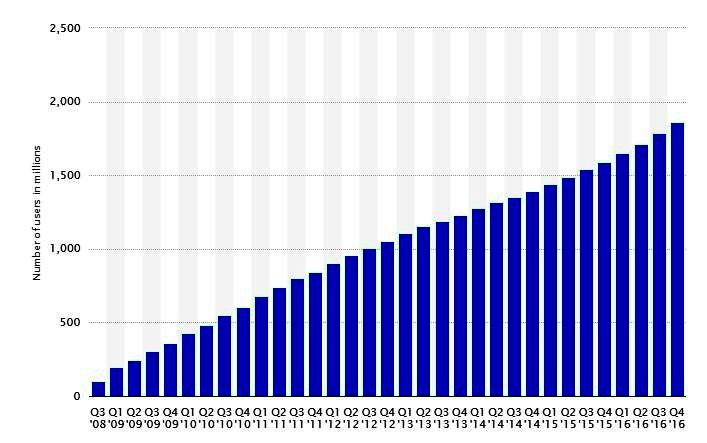
\includegraphics[scale=0.7]{fb.jpg}
  \caption[Number of Monthly Active Facebook Users World wide as of 4th Quarter 2016 (in millions)]{ Number of monthly active facebook users worldwide as of 4th quarter 2016 (in millions)[6]}
   \label{fg}
 
\end{figure}
\noindent
We know that Face book is the most popular social networking site at present. Number of monthly active Facebook users worldwide as of 4th quarter 2016 (in millions)is shown in figure 1.1. This statistic shows a timeline with the worldwide number of monthly active Facebook users from 2008 to 2016. As of the fourth quarter of 2016,which is showed in X -coordinate, Facebook had 1.86 billion monthly active users,which is showed in Y-coordinates. Active users are those which have logged in to Facebook during the last 30 days.  Every day, people add more than 100 million tags to photos on Facebook.At present around 350 billion photos are uploaded in facebook.so secure computing is an  important domain at present[6].

%% % \nointent
  \vspace*{1pc}
In software engineering, dependability is the ability to provide services that can defensibly be trusted within a time-period and  is a measure of a system's reliability, safety and security. Secure computing deals with Computer security, also known as cyber security  or IT security is the protection of computer systems from the theft or damage to the hardware, software or the information on them, as well as from disruption or misdirection of the services they provide today.The field is of growing importance due to the increasing reliance on computer systems and the Internet in most societies, wireless networks such as Bluetooth and Wi-Fi and the growth of "smart" devices, including smart phones, televisions and tiny devices as part of the Internet of Things.
\subsection[Facial Recognition]{Facial Recognition}
Facial recognition(FR) technology once seemed like something out of the movies, but it is increasingly being incorporated into our everyday lives. Both public and private sector organizations are incorporating facial recognition into products and services to create substantial benefits for consumers. As with any new technology, innovative capabilities can present new or expanded privacy risks. Facial recognition data is personal and sensitive, making privacy an important challenge for companies[3].  Commercial use of facial recognition technology raises many of the same security concerns applicable to sensitive personal information generally.  social networks and other large databases of identified individual images could increasingly become the targets of access by unauthorized individuals, leading to consumers’ facial recognition data being used in ways that consumers cannot anticipate or control, and without their knowledge. CBIR , Content Based Image Retrieval has been a significant area of research in the last few decades[8]. 
%\begin{enumerate}
%\item item1
%\item item2..
%\end{itemize}
%\paragraph{} Paragrahs are separated like this
%\paragraph{} And like this

%Images are added like this
%\begin{figure}[hbtp]
%\centering
%\includegraphics[scale=.2]{crn.png} 
%\caption{Basic working of CRN }
%\end{figure}
%\section{A New Section}
%\justifying
%\paragraph{}
%A new section is added like this. You can have subsections and subsubsections the same way
%\subsection{A Subsection}
%\justifying
%\paragraph{}
%A subsection is added like this
%\subsubsection{A subsubsection}
%\justifying
%\paragraph{}
%A subsubsection is added like this
%\section{Contributions}
%Contributed slight modifications to the system such that it can be implemented in the college central library.
%What contributions have you given to this work. What have you added to project other than your base paper.
\section[Objective]{\fontsize{14}{12}\selectfont OBJECTIVE}
Photo giving out is one of the most well-liked features in online social networks such as Facebook. Lamentably, imprudent photograph posting may uncover security of people in a posted photograph. Main objective of the system is preventing the possible privacy leakage issue related to group photo uploading in social networks. To establish this every co-photo owners should participate in the decision making of photo posting. The system can solves the subject of posting group photos on a social network by sending a notification to co photo owners regarding their presence. If the entire co-photo owner then the s are accepting the notification, the group photo will be uploaded otherwise the photo will be rejected.  We assume that each user u has a privacy policy$ Pu(i)$ and an exposure policy $Eu(i)$ for a specific photo$ i$. The privacy policy$ Pu(i)$ indicates the set of users who can access photo$ u $and exposure policy$ Eu(i)$ indicates the set of users who can access$ i$ when user$ u$ is involved[1]. One of the main objectives is to get an   efficient FR system for this project. If the photo co-owner is not login to the social network he or she is unable to see the notification and the group photo cannot be uploaded for long. To solve this issue it is possible to set a time limit, for example 2 days or 3 days.If it is set 3 days time limit after that photo will be uploaded automatically. More over for the photo co-owners safety it is possible to send SMS regarding the photo uploading and time limit, so they can login and either accept or reject the notification.. To do all of this we need a good FR system.  One of the main objectives is to get an   efficient FR system for this project . This system is using CBIR (content based image retrieval) algorithm with K-mean clustering for training images and face recognition[12].
\section[Scope]{\fontsize{14}{12}\selectfont SCOPE}
A method is proposed to empower people conceivably in a photograph to give the consents before posting a co-photograph. A security protecting FR framework is outlined to distinguish people in a co -photograph. The proposed framework is highlighted with low calculation expense and classification of the preparation set. Hypothetical investigation and analyses were directed to show adequacy and proficiency of the proposed plan. We expect that our proposed plan be extremely helpful in ensuring clients' security in photograph/picture sharing over online informal communities. Then again, there dependably exist exchange off in the middle of protection and utility. We show that our system is superior to  other possible approaches in terms of recognition ratio and efficiency. Expect that this proposed scheme would be very useful in protecting users’ privacy.
\section[Scheme]{\fontsize{14}{12}\selectfont SCHEME}
\textbf{Chapter 1} This thesis is organized in such a way that, Chapter 1 includes the introduction section which explains Introduction including General Background, Objective, Scope, Scheme of project work etc.\\
\textbf{Chapter 2} is about the literature survey.This chapter gives a brief survey done on control of photo sharing on online social networks.\\
\textbf{Chapter 3} briefs the problem associated with the existing system.\\
\textbf{Chapter 4} covers the proposed system \\
\textbf{Chapter 5} covers task setup and implementation.\\
\textbf{Chapter 6} deals with results and discussion.\\
\textbf{Chapter 7} includes conclusion and future enhancement.\\
%%%%%%%%%%%%%%%%[ LITERATURE SURVEY ]%%%%%%%%%%%%%%%%
\addtocontents{toc}{\cftpagenumberson{chapter}}
\chapter[LITERATURE SURVEY]{\fontsize{16}{12}\selectfont LITERATURE SURVEY}
%Give a detailed description of the literature review. Give appropriate citations. Each paper can be given a separate section\\
Photo sharing is probably the most popular feature in online social networks such as Facebook. Unfortunately, careless photo posting may reveal privacy of individuals in a posted photo. The things become more difficult when it is added much functions like photo uploading and tagging. For instance, these days we can contribute to any picture as we like on OSNs, in spite of whether this photograph contains other populace (is a co-photo) or not.This section first two papers discuss various security issues and the available prevention methods  related to group photo uploading , and the following  papers  discuss about the Haar cascade classifier used for face detection,face recognition system and  CBIR algorithms  used for the face recognition system. For  the efficient  working of this system a good FR system is needed. 
\section[Moving Beyond Un Tagging: Photo Privacy in a Tagged World]{\fontsize{14}{12}\selectfont MOVING BEYOND UN TAGGING: PHOTO PRIVACY IN A TAGGED WORLD }
Social networking users unknowingly reveal certain kinds of personal information that malicious attackers could profit from to perpetrate significant privacy breaches. This section quantitatively demonstrates how the simple act of tagging pictures on the social networking site of Facebook could reveal private user attributes that are extremely sensitive. Our results suggest that photo tags can be used to help predicting some, but not all, of the analyzed attributes. We believe our analysis make users aware of significant breaches of their privacy and could inform the design of new privacy-preserving ways of tagging pictures on social networking sites.
The ability to upload and share photo albums on Facebook was launched in October 2005, when the site had about 5 million users . By then, photo hosting was already exploding on the Internet and other sites which offered photo hosting services were already quite popular, like MySpace and Flickr .Facebook user growth is increasing day by day. There are currently almost 90 billion photos total on Facebook.%Facebook subscribers in the world by region-June 2016 is shown in fig 2.
Number social networking  of subscribers are increasing day by day thus privacy leakage issues also increasing especially while uploading photograph. Photo tagging is a popular feature of many social network sites that allows users to annotate uploaded images with those who are in them, explicitly linking the photo to each person’s  profile.
%\begin{figure}[h]
% \centering
 % \includegraphics[scale=1]{fb1.jpg}
 % \caption[Facebook subscribers in the world by region-June 2016]{ 5Facebook subscribers in the world by region-June 2016 \cite{base1}}
%  \label{table1}
%\end{figure}     
Every day, people add more than 100 million tags to photos on Facebook. That's the number Facebook provides before activating semi automated photo tagging by facial recognition.  In this document, it is inspected confidentiality concerns and mechanisms regarding this tagged photograph. Using a focal point of group, we explored the requirements and concerns of users, follow-on in a set of design considerations for tagged photograph confidentiality[2],[4],[6].

%% % \nointent
  \vspace*{1pc}
Now Facebook added the new security to prevent the privacy leakage issue due to photo tagging, people can set “review the tag before appearing the time line option “.but still people can share the photo because somebody is uploading the photo first without taking the co- photo owner’s permission so even the review tag options is available,  it  is not preventing co-photo owner’s privacy. 
\section[Multy Party Privacy Risks In Social Networks]{\fontsize{14}{12}\selectfont MULTI-PARTY PRIVACY RISKS IN SOCIAL NETWORKS}
Most social media users consistently criticize mainstream social media for providing very complex privacy controls. These are often too difficult to understand, require time-consuming manual configuration, and do not allow for appropriate privacy management. Users are required to set many privacy controls . This makes most users unable to cope with the complexity of privacy management in social media, which has led to numerous incidents in which people have lost their jobs, have been cyber bullied, or have lost court cases due to the inappropriate communication of personal information through social media. Empirical evidence shows that  this  significantly  discourages  users  to  either  join  social media  or  to  show  high  engagement  when  they  join in terms of how much they participate in social media sites, e.g., the  amount  of  photos  they  upload. In this section, we examine how the lack of joint privacy controls over content can inadvertently reveal sensitive information about a user including preferences, relationships, conversations, and photos.

%% % \nointent
  \vspace*{1pc}
This slow erosion of personal privacy can be prevented by the adoption of multi party privacy controls. The current lack of multi party privacy results in scattered references to users throughout social networks that can be collected by adversaries who have the resources, sophistication, and motivation to glean as much information from social networks as possible[9],10],[19]. 

%% % \nointent
  \vspace*{1pc}
Here user can decide how many want to give the access permission to share the group photo, so user  can select a group of people before uploading a group photo, those are allow to access and share the group photo or user can select certain people and deny  their access and share permission of a group photo. This is also one of the prevention method of privacy leakage issue but still a single conflict may pose a minimal risk to privacy and  still it is not preserving the co-photo owners privacy.
\section[Rapid Object Detection Using A Boosted Cascade Of Simple Features]{\fontsize{14}{12}\selectfont RAPID OBJECT DETECTION USING A BOOSTED CASCADE OF SIMPLE FEATURES}
Face detection algorithms detects faces and determines the precise face area and exposure conditions. Automatically crops images or sets the proper exposure conditions for optimum results. There are many methods used for face detection.A few methods are showm in table 2.1. Those are First automated system, PCA, Eigenface, Fisherface and AdaBoost+HaarCascade .Out of this Haar cascade classifier is a well used classifier for face detection.
%%%%%%%%%%%%%%%%%%%%%%%%%%
\begin{table}[H]
\centering
\caption{Face detection methods }
~\\
\label{tb1}
\begin{tabular}{|c|c|c|}
\hline
\textbf{Year:} &\textbf{Author}       &\textbf{Methods}  \\
\hline
1973     &Kande    &   First automated system     \\
      
\hline
1987 &Sirovich and Kirby&Principal Component Analysis           \\
 \hline
1991 &Turk and Pentland&Eigenface           \\


\hline
1996     &Etemad and Chellapa   &   Fisherface     \\
      
\hline

2001 &Viola and Jones&AdaBoost+HaarCascade           \\

\hline
\end{tabular}
\end{table}
%%%%%%%%%%%%%%%%%%%%%
\noindent
Haar cascade classifier is  trained with a lot of face images and non face  images.Initially more than 160000+ features values are used within a detector at 24x24 base resolutions which need to be calculated.  For this Haar features shown in the Figure 2.1 is used. Each feature  is a single value which is calculated by subtracting the sum of pixels in white rectangle from the sum of pixels in  black rectangle. To reduce the computation cost used the concept integral image. Most of the features among 160000+ features are not relevant so used Adaboost algorithm to find out the relevant features. To do this every features apply to training image and elected the features with minimum error rate .After these are found a weighted combination of all features are used n evaluating and deciding the given window has a face or not Each feature is called a week classifying Adaboost construct a strong classifier as a linear combination of these week classifier.
 \begin{figure}[H]
 \centering
  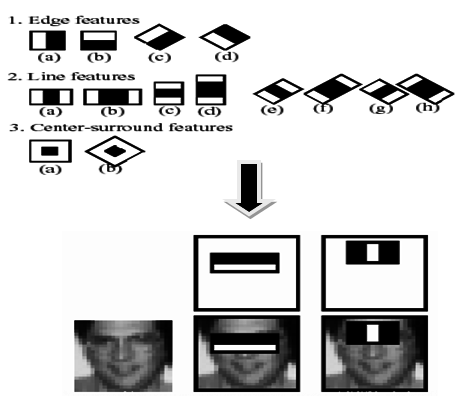
\includegraphics[scale=0.8]{haar.png}
  \caption[Haar features for face detection]{ Haar features for face detection[14]}
  \label{haar}
\end{figure}
\noindent
Cascade classifier composed of different stages and each stage has certain no of features.Each stage is used to determine a given sub windows face or not. The sub window is immediately discarded if it is not a face.

%% % \nointent
  \vspace*{1pc}
Face detection using Haar cascade classifier is very fast, it has an efficient feature selection still there will be error or miss classification.100 percentage accuracy cannot be ensured[14].
%---------------------------------------------------------------------------------------------
\section[Face Recognition for Improved Face Annotation in Personal Photo Collections Shared on Online Social Networks ]{\fontsize{14}{12}\selectfont  FACE RECOGNITION FOR IMPROVED FACE ANNOTATION IN PERSONAL PHOTO COLLECTIONS SHARED ON ONLINE SOCIAL NETWORKS}
\noindent
Using face annotation for effective management of personal photos in online social networks (OSNs) is currently of considerable practical interest. In this paper, we propose a novel collaborative face recognition (FR) framework, improving the accuracy of face annotation by effectively making use of multiple FR engines available in an OSN. In particular, our collaborative FR framework consists of two major parts: selection of FR engines and merging (or fusion) of multiple FR results. The selection of FR engines aims at determining a set of personalized FR engines that are suitable for recognizing query face images belonging to a particular member of the OSN. For this purpose, we exploit both social network context in an OSN and social context in personal photo collections. In addition, to take advantage of the availability of multiple FR results retrieved from the selected FR engines, we devise two effective solutions for merging FR results, adopting traditional techniques for combining multiple classifier results. Experiments were conducted using 547,991 personal photos collected from an existing OSN[3].

%% % \nointent
  \vspace*{1pc}
Our results demonstrate that the proposed collaborative FR method is able to significantly improve the accuracy of face annotation, compared to conventional FR approaches that only make use of a single FR engine. We demonstrate that our collaborative FR framework has a low computational cost and comes with a design that is suited for deployment in a decentralized OSN. Accuracy is high in  collaborative FR system but it is time consuming and 100 percentage  face recognition is not ensure here.
\section[Color and Texture Features for Content Based Image Retrieval]{\fontsize{14}{12}\selectfont  COLOR AND TEXTURE FEATURES FOR CONTENT BASED IMAGE RETRIEVAL}
CBIR, Content Based Image Retrieval has been an important area of research in the last few
decades. A retrieval mechanism using color and texture is being proposed here. Depending on the characteristic of the image texture, it can be represented by multi wavelet transform. The color correlogram in the RGB color space is chosen as the color feature. The main motivation of this system is to use the Multi Wavelet decomposition scheme and color correlogram, which yield improved retrieval performance. Through the combination of Multi wavelet decomposition and color correlogram we can increase the number of features, which in turn improves the retrieval accuracy. To support the efficient and fast retrieval of similar images from image databases, feature extraction plays an important role. The technique used for comparing images plays the fundamental ingredient of content based image retrieval.

\subsection[Color Correlogram]{Color Correlogram}
A new feature for color retrieval is the color correlogram.This feature only captures spatial
correlation between identical colors, that is, it characterized how the spatial correlation of pairs of color changes with distance in an image.
\subsection[Multi Wavelet Transform]{Multi Wavelet Transform}
Multi Wavelets are defined using several wavelets with several scaling functions. The base
features for this transform include compact support, Orthogonality, symmetry, and high order
approximation . A scalar wavelet cannot possess all these properties together at the same time, whereas a multi wavelet can can simultaneously provide perfect representation while preserving length, good performance at the boundaries , and a high order of approximation . Therefore, Multi wavelets offers superior performance and high degree of freedom for image processing applications, compared with scalar wavelets[11],[18].
%%%%%%%%%%%%%%%%%
\begin{enumerate}
\item Texture Feature Extraction
\begin{enumerate}
\item  Convert all database images into gray images.
 \item Decompose each image in the Multi wavelet domain.
\item  Compute the standard deviation σ k on each sub-band of the Multi Wavelet decomposed
image.
\item  The resulting SD vector is 
%$f$ = [ \sigma 1, \sigma2, \sigma 3, ..., \sigma k ]
 
\end{enumerate}

\item Color Feature Extraction
\begin{enumerate}
\item Load the image.
\item Separate the R, G, and B spaces from the image.
\item Quantize the each color space into 32 levels .
\item Apply the correlogram in 0 $^{\circ}$   , 45 $^{\circ}$  , 90 $^{\circ}$  , and 135 $^{\circ}$  on each color space.

\item Construct the feature vector by using correlogram
\end{enumerate}

\item Combined Feature
Form the combined feature vector by concatenating the color feature and texture feature.
\item Apply query image and calculate the combined feature vector.
\item Calculate the similarity using Euclidean distance.
\begin{equation}
D^{E}_{qi} = \sqrt{\left(\overline{f_q }-\overline{f_i}\right)^2}
\end{equation}
\item Retrieve all relevant images to query image based on minimum Euclidean distance.
\end{enumerate}
%% \nointent
The main advantage of wavelet decomposition is that it yields a large number of sub bands. which in turn improves the retrieval accuracy. A major disadvantage of this technique is its limitation in feature set.

%------------------------------------------------------------------------------
\section[CBIR Based Image Retrieval Using Modified Haar Wavelet Transform and K Mean Clustering]{\fontsize{14}{12}\selectfont  CBIR BASED IMAGE RETRIEVAL USING MODIFIED HAAR WAVELET TRANSFORM AND K MEANS CLUSTERING}
\subsection[Content Based Image Retrieval]{Content based image retrieval}
\noindent
To retrieve any image, we have to search for it among the database using some search engine. Then, this search engine will retrieve many of images related to the searched one. The main problem encounters user here is the difficulty of locating his relevant image in this large and varied collection of resulted images. This problem referred to as image retrieval problem.The earlier approach for image retrieval is text-based, in which images are indexed using keywords, subject headings, or classification codes which in turn are used as retrieval keys during search and retrieval. Unfortunately, for the large database the difficulties faced by text-based retrieval became more and more severe and the process becomes very laborious and time consuming task.

%% % \nointent
  \vspace*{1pc}
To overcome these problems and others, the image contents, features of the image, like color, texture and shape that are automatically extracted from the images themselves have been used for image retrieval. This method is called content-based image retrieval (CBIR) [7]. CBIR enables the elimination of the difficulties that exist in traditional text-based query for large image database and then the system will provide better indexing and return more accurate results.
"Content-based" means that the search will analyze the actual contents of the image rather than the metadata such as keywords, tags, and/or descriptions associated with the image. The term 'content' in this context might refer to colors, shapes, textures, or any other information that can be derived from the image itself[16],[17].

%% % \nointent
  \vspace*{1pc}
Existing system explain the image retrieval using CBIR with Haar wavelength transformation[12],[15]. System Architecture of CBIR system is shown in Figure 2.2.It has mainly two phases, indexing and searching. Indexing includes decomposition, feature extraction and clustering and another one is searching for a query image. It is an image retrieval technique using Modified Haar Wavelet Transform and K Means Clustering First process is image training including decomposition, feature extraction and clustering. In the searching phase the most similar images to the query image [12], from the cluster files can be retrieved using CBIR image retrieval algorithm[8].
 \clearpage 
 \vspace{1pc}
 \vspace{1pc}
\begin{figure}[ht]
\begin{minipage}[c]{1\linewidth}
\begin{center}
 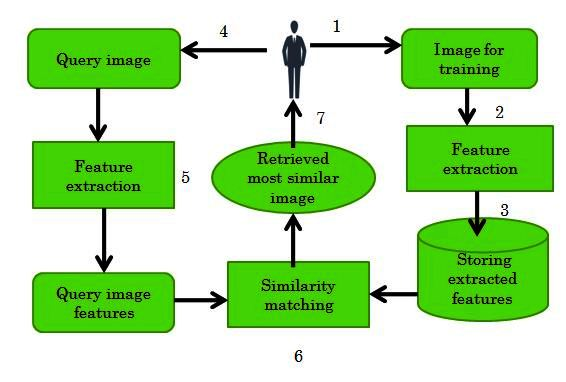
\includegraphics[width=\textwidth]{e.jpg}
           % \text{\scriptsize(ISO 9001:2008 Certified)}
            \caption[Architecture of existing system]{Architecture of existing system (CBIR)[12]}
             \label{Invite friends}
\end{center}
\end{minipage}
\end{figure}
\noindent
\vspace{1pc}
\subsection[CBIR Algorithm:]{CBIR Algorithm:}
\begin{algorithm}
\caption{CBIR Algorithm to  retrieve most similar image for query image}
   Input: Query image\\
   Output:Most similar images to  the input image\\
\begin{algorithmic}[1]
\State Give input image
\State Extract the feature vector for the input image 
\State Calculate the weighted features vectors for the input image
\State Calculate the distance between the input image and the centroid            of each K-mean  cluster  and find  the smallest distance

\State Calculate the distance between the input image and the images
            in the cluster that has the smallest distance with
             the    input image

\State Retrieve   most similar images to the input image

\end{algorithmic}
\end{algorithm}
\clearpage
\noindent
The main unit of CBIR is an image retrieval technique that used to retrieve from the database the most similar images to the query image [12]. A typical content-based retrieval system is divided into off-line feature extraction and online image retrieval. In off-line stage, the system automatically extracts visual attributes at either a low-level (such as color, texture, and shape) or at a high-level (such as a color histogram), or both for each image in the database based on its pixel values and stores them in a different database within the system called a feature database [17]. The feature data (also known as image signature) for each of the visual attributes of each image is very much smaller in size compared to the image data. . A Haar Wavelet transform decomposes an image into two components: average and difference.Each color in the image can be represented by considering the pixels as a point in space and from this matrices for each Red, Green and Blue components of RGB are constructed. Once decomposition over  calculate feature vector  based on F-norm theory storing the values to cluster files for future use.
\subsection[K-Means for Clustering ]{K-Means for Clustering }
\noindent
The time of image retrieval in almost all CBIR systems depends in a large degree on the number of images in the database. Many existing systems attempt to compare the query image with every target image in the database to find the top matching images, resulting in an essentially linear search, which is highly computationally inefficient when the database is large. However, it is a benefit to use all images in the database for similarity matching, so that the results will be good enough. To overcome this problem, image clustering or categorization has often been treated as a preprocessing step to speed-up image retrieval in large databases and to improve the accuracy so that when a query is received, only a part of the database needs to be searched, while a large portion of the database may be eliminated in the search. This certainly saves significant query processing time without compromising the retrieval precision. Clustering algorithms are used as a preprocessing step, performed offline, to cluster the database into N different categories and each feature vector, along with its associated class number, is recorded in the database files. 
The basic step of k-means clustering is simple. In the beginning, determine number of cluster K and assume the centroid or center of these clusters. We can take any random objects as the initial centroids or the first K objects can also serve as the initial centroids. Then the K means algorithm will do the three steps below until convergence.

%% % \nointent
  \vspace*{1pc}
Clustering is very efficient and powerful technology to handle large data sets. It assists faster image retrieval and also allows the search for most relevant images in large image database [16]. K-means is a clustering method which is known for its efficiency in producing accurate results in image retrieval. By using k-means user can select the closer group of image so that they get fast result. 
Finally, query image is the image the user is interested in and wants to find similar images from the image database. The feature vector for the query image is extracted and is now compared with the image clusters. Based on minimum Euclidean distance, the target image cluster closest to the query image is retrieved from the database.\\
In the proposed system, we use k-means algorithm to classify the feature vectors of the input images. We select the k-means algorithm because it is suitable to cluster large amount of data. Each feature vector is treated as an object having a location in space. The cluster generates in which objects within this cluster are close to each other and far from objects in other clusters as possible. Selecting the distance measure is an important step in clustering. The distance measure determines the similarity of two images. 
A cluster is a group of objects that are similar to each other within the same group and are dissimilar to the objects in other groups. Clustering has been widely used in different applications, including pattern recognition, data analysis, machine learning, and image processing. K-means is one of the simplest clustering algorithms. In k-means algorithm, the clustering results are measured by the sum of within-cluster distances between every vector and its cluster centroid. This criterion ensures that the clusters generated are tight. K-means algorithm takes k, the number of clusters to be generated, as the input parameter and partitions a set of N objects into k clusters so that the resulting intra-cluster similarity is high but the inter-cluster similarity is low. If the number of clusters is not specified, a simple method is done. The algorithm initializes the number of clusters to a certain number less than the total number of the dataset. The algorithm increases that number gradually until the average distance between a vector and its cluster centroid is below a given threshold [12].

%% % \nointent
  \vspace*{1pc}
The k-means algorithm works as the following. The number of clusters, k, is entered as an input parameter. The algorithm randomly selects k of the objects, each of which initially represents a cluster centroid. The centroid for each cluster is a point to which the sum of distances from all objects in that cluster is minimized. For each of the remaining objects, an object is assigned to the cluster to which it is most similar.
\section[Performance Analysis of Existing System]{\fontsize{14}{12}\selectfont PERFORMANCE ANALYSIS OF EXISTING SYSTEM}
%\noindent
This section, analyse the overall performance of the existing system by computing the
performance score for each module in the system. The performance analysis graph is shown in Figure 2.3 The modules used for the performance analysis  are image training and  face recognition. Then plot the performance graph with time in seconds.The time taken to run each module is added in the given table 2.2, which is the observation table for CBIR algorithm.
\\ 
%\begin{figure}[h]
%\begin{minipage}[c]{.5\linewidth}
%\begin{center}
% 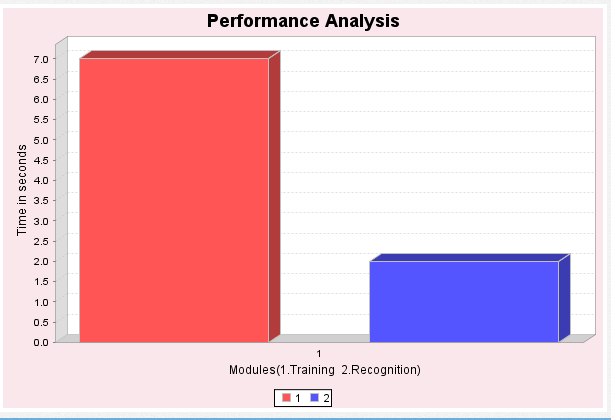
\includegraphics[width=\textwidth]{cbir.png}
           % \text{\scriptsize(ISO 9001:2008 Certified)}
          %  \caption[Invite friends]{Performance analysis of existing system}
            % \label{Invite friends}
%\end{center}
%\end{minipage}
%\end{figure}
%%%%%%%%%%%%%%%%%%%%%%%%%%%%%%%%% 
 \begin{figure}[h]
 \centering
  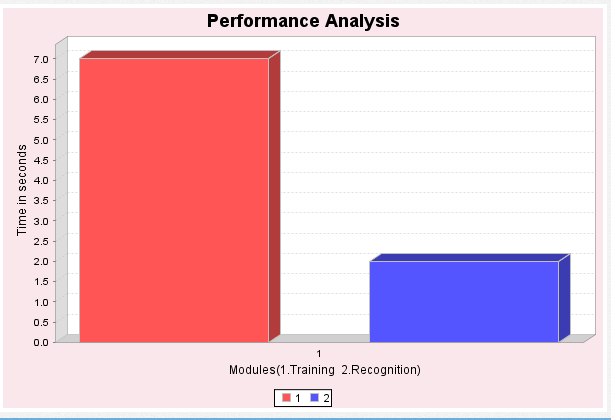
\includegraphics[scale=0.6]{cbir.png}
  \caption[Performance Analysis of Existing System]{ Performance analysis of existing system}
  \label{table1}
\end{figure}
\vspace{1 cm}

%%%%%%%%%%%%%%%%%%%%%%%%%%%%%%%%%%
\begin{table}[H]
\centering
\caption{Observation table for CBIR algorithm }
\label{routing}
\vspace{.5 cm}
\begin{tabular}{|c|c|c|}
\hline
\textbf{SNO:} &\textbf{Modules}       &\textbf{Time taken(seconds)}  \\
\hline
1     &Training    &   7      \\
      
\hline
2 &Face Recognition&2            \\
\hline
\end{tabular}
\end{table}
\clearpage
%%%%%%%%%%%%%%%%%%%%%%%%
%-----------------------------------------------------------------------------------------------
%%%%%%%%%%%%%%%%%%%%%%%%%%%%%[ PRROBLEM DEFINITION ]%%%%%%%%%%%%%%%%%%%%%%%%%%
\addtocontents{toc}{\cftpagenumberson{chapter}}
\chapter[PROBLEM DEFINITION]{\fontsize{16}{12}\selectfont PROBLEM DEFINITION}
\noindent
In a typical CBIR system, low- level visual image features that is colour, texture, and shape are automatically extracted for image descriptions and indexing purposes. To search for desirable images, a user presents an image as an example of similarity, and the system returns a set of similar images based on the extracted features  The main issue with CBIR system is the time of image retrieval in almost all CBIR systems depends in a large degree on the number of images in the database.

%% % \nointent
  \vspace*{1pc} 
Two main issues with CBIR systems are efficiency and accuracy. Hence, an effective CBIR system needs to have an efficient search mechanism and also accurate set of features. Out of all the mechanisms used in CBIR, k-means clustering is found to have better efficiency and accuracy. 
"Content-based" means that the search will analyze the actual contents of the image rather than the metadata such as keywords, tags, and/or descriptions associated with the image. The term 'content' refer to colours, shapes, textures, or any other information that can be derived from the image itself.
 CBIR is desirable because most web based image search engines rely purely on metadata and this produces a lot of garbage in the results. Also having humans manually enter keywords for images in a large database can be inefficient, expensive and may not capture every keyword that describes the image.
 
 %% \nointent
  \vspace*{1pc}
   Thus system that can filter images based on their content would provide better indexing and return more accurate results. Again the performance of the CBIR system is improved by using K-Means clustering technique .If we are using CBIR to train individual’s images and for face recognition in our proposed system. To get enough training sample is actually little difficult task, so FR engine may be unsuccessful to identify the faces of each individual in a group photo.FR engine could be trained to recognize social friends (people in social circle) but to get enough training sample is a difficult task.To get efficient result CBIR demands more training samples (photos of each specific person), but online photo resources are often insufficient, also with varying poses and facial expressions CBIR system may fail to recognize the faces of each individual in a group photo. More demanding privacy setting may limit the number of the photos publicly available to train the FR system..Another major issue we are facing is large number of users are absent for us to carry out the network-wide evaluation. We simulate a real-life social network with the small-world network.
 \clearpage
%%%%%%%%%%%%%%%%%%%%%%%[ MODIFICATION ]%%%%%%%%%%%%%%%%%%%%%%%%%%%%%%
\addtocontents{toc}{\cftpagenumberson{chapter}}
\chapter[METHODOLOGY]{\fontsize{16}{12}\selectfont METHODOLOGY}
\noindent
The proposed system is used to reduce the privacy leakage issues while uploading a photo through OSNs.CBIR algorithm is used for face recognition in the proposed system.CBIR algorithm is one of the most popular algorithm used for image retrieval.CBIR system  defines the similarity between contents of two images based on global feature(i.e. features extracted from the whole image).The proposed system  using Haar cascade classifier for face detection,it crops all the face regions from the images ,so need not find the similarity based on global feature.

 %% \nointent
  \vspace*{1pc}
  To curb the privacy leakage, we proposed to enable individuals potentially in a photo to give the permissions before posting a co-photo. We designed a privacy preserving Content based image retrieval FR system to identify individuals in a co-photo.Face detection is an important part in the proposed system because in the proposed system each co-photo owners are participating in the decision making of photo uploading through social networks.\vspace{1 pc} The proposed system is featured with low computation cost and confidentiality of the training set.  The proposed system added time limit for notification acceptance, and SMS notification to inform the co-photo owner about the time limit for notification. We expect that our proposed scheme be  very useful in protecting users’ privacy in photo/image sharing over online social networks.
\section[Proposed System Architecture]{\fontsize{14}{12}\selectfont PROPOSED SYSTEM ARCHITECTURE}
%\subsection[Admin]{Admin}
\begin{figure}[H]
\begin{minipage}{1\linewidth}
\centering
\begin{center}
 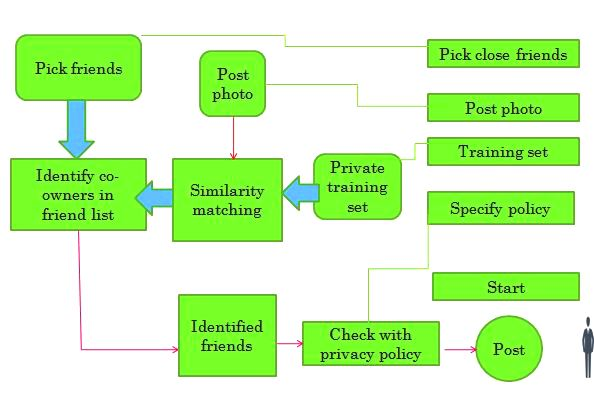
\includegraphics[width=\textwidth]{p.jpg}
           % \text{\scriptsize(ISO 9001:2008 Certified)}
            \caption[Proposed System Architecture]{Proposed system Architecture}
             \label{Invite friends}
\end{center}
\end{minipage}
\end{figure}
%\clearing
\subsection[Start]{Start}
%\noindent
%4.1.1Start
User can register to Online Social Network by entering the details like name, DOB, gender, Email, mobile number, user name, password etc. Once registered successfully user can login to his/her account. User or admin can login to this system if they have a valid user id and password. Admin can login with a valid password, once login admin can view the user details. Main function of admin is to train the user image
\subsection[Specify Policy]{Specify policy}
%\noindent
%4.1.2 Specify policy
We assume that each user u has a privacy policy$Pu(i)$ and a exposure policy $Eu(i)$ for a specific photo$ i$. The privacy policy $Pu(i)$ indicates the set of users who can access photo$ i $
.In our project we set two options ,one is view public and net is view my friends.If a user is selecting public option ,once photo is uploaded  that photo will be shown publically ,if he/ she is setting only my friends option then once the photo is  uploaded ,it  will be available in the time line of his/her friends home page.Exposure policy $Eu(i)$ indicates the set of users who can access$ i$ when user $u$ is involved.In our project we limited this within the close friend list. According to our scheme, this friend list should be intersection of owner’s privacy policy and co-photo owners’ exposure policies. At present, when the push button “Post Photo” is pressed, co-owners of$ i$ are identified, and then notifications along with $i$ are sending to the co-owners  within the close friend list to request permissions. If they all agree to post$ i$, $i$ will be shared on the owner’s page like a normal photo. In this sense, users could specify their privacy policy but their exposure policies are depends the set of users who can access $i$ when user $u$ is involved.
\subsection[Training]{Training}
%\noindent
%4.1.3 Training
A log in/out button could be used for log in/out with our social network site. After login , user can train their individual images , we need an efficient content based image retrieval facial recognition (FR) system that can used to train users images. We are using Haar cascade classifier for face detection and CBIR algorithm to train individual’s images and for face recognition.  FR engine could be trained to recognize social friends (people in social circle) but to get enough training sample is a difficult task.
 
 %% \nointent
  \vspace*{1pc}
FR engine with advanced recognition ratio demands more training samples. In the training phase, both decomposition and feature extraction takes place. Haar Wavelet Transform is used for calculating the feature vectors, weighted feature vector represented as weight function w(). Then k-means clustering algorithm is used for clustering the images based on their feature vectors , considering the minimum Euclidean distance. The basic idea is to transfer an image into matrix in which each element of the matrix represents a pixel in the image. A Haar Wavelet transform decomposes an image into two components: average and difference.Each color in the image can be represented by considering the pixels as a point in space and from this matrices for each Red, Green and Blue components of RGB are constructed. This is then decomposed into four sub matrices through row and column transformations[Appendix-A].
 % \thispagestyle{empty
%\begin{enumerate}[label=(\roman*)]
\begin{description}
\item[(i)]  The formula for calculating average and difference at level 1 is given by
%The formula for calculating average at level 1 is given by}
%\end{enumerate}
The formula for calculating average is shown in equation(4.1):
\begin{equation}\label{}
avg = \frac{f_n+f_{n+1}}{\sqrt{2}}, \text{where n} = 1,2,3,.....\frac{n}{2}
\end{equation}

And difference at the same level is shown in equation(4.2):
\begin{equation}\label{}
diff = \frac{f_n-f_{n+1}}{\sqrt{2}},\text{where n}=1,2,3,.....\frac{n}{2} 
\end{equation}
%\thispagestyle{empty}
%\begin{enumerate}(ii)

\item[(ii)]To calculate the Haar transform of an array of n samples: 
%\end{enumerate}
       \begin{enumerate}
 \item Find the average of each pair of samples. (n/2 averages) 
 \item  Find the difference between each average and the samples it was calculated from. (n/2 differences) 
 \item  Fill the first half of the array with averages 
 \item  Fill the second half of the array with differences. 
 \item Repeat the process on the first half of the array. While doing this the array size should be power of two.
\end{enumerate}
\end{description} 
This steps are repeated for both row and column. Once the process is completed, the matrix gets decomposed into four sub-matrices each of dimension (number of rows/2) x (number of
columns/2) and is called A, H, V and D respectively. A (approximation area) contains
information about the analyzed image’s global properties, H (horizontal area) contains
information about vertical lines hidden in the image, V (vertical area) contains information about the horizontal lines hidden in the image and D (diagonal area) contains information about the diagonal details hidden in the image.
%\begin{enumerate}(ii)
\begin{description}
\item[(iii)] The advantages of Haar Wavelet transform: 
%\end{enumerate}
\begin{enumerate}
\item  Best performance in terms of computation time 
\item Computation speed is high 
\item Simplicity 
 \item HWT is efficient compression method
\end{enumerate}
\end{description} 
Once decomposition is done, then feature vectors can be constructed using mean and standard
deviation of energy distribution ( $F$-norm) of each sub-band at each level. The equation for calculating $F$-norm  is shown in equation(4.3)
Given a square matrix$A$ and $A_i$ is  a sub matrix from it, then $F$- norm given by,
\begin{equation}
|A_i|_{F} =\left[ \sum\limits_{k=1}^i \sum\limits_{k=1}^i|a_{kl}|{^2} \right]^{\frac{1}{2}}
\end{equation}
The equation for calculating mean($\mu$)is shown in equation(4.4)
 \begin{equation}
%\text{Mean($\mu$)}=\frac{\sum \text{F-norm}}{\text{no of columns of F-norm}}}
\end{equation}
The equation for calculating standard deviation($\sigma$)is shown in equation(4.5)
 \begin{equation}
\text{StanderdDeviation($\sigma$)} = \sqrt{\frac{\sum \left(\text{F-norm}- mean\right)^2}{\text{no of columns of F-norm}}}
\end{equation}
The equation for calculating variance($\sigma^{2}$)is shown in equation(4.6)
 \begin{equation}
\text{Variance($\sigma^{2}$)} = \Bigg(\sqrt{\frac{\sum \left(\text{F-norm}- mean\right)^2}{\text{no of columns of F-norm}}}\Bigg)^{2}
\end{equation}

 %%%%%%%%%%%%%%5
 \begin{description} 
 \item[(iv)]K Mean Algorithm
 %\end{description}  
The basic step of k-means clustering is simple. In the beginning, determine number of cluster K and assume the centroid or center of these clusters. We can take any random objects as the initial centroids or the first K objects can also serve as the initial centroids. Then the K means algorithm will do the three steps below until convergence[12].
    % \begin{enumerate}
    % \item aaaaaaaaaaaaaaaaaaaaaaaaaaaaa
     %\item bbbbbbbbbbbbbbbbbbbbbbbbbbbb
     %\item cccccccccccccccccccccccccccccc
    % \end{enumerate}
     \end{description}     
      \begin{algorithm}
\caption{K-Mean  Algorithm }
   Input: Number of cluster k,N objects\\
   Output:A set of K clusters\\
\begin{algorithmic}[1]
\State Arbitrarily choose k objects as the initial cluster centers.
\State (Re)Assign each objects to the cluster to which the object is the most similar based on the mean value of objects in the cluster.  
\State Update the cluster means,i.e, calculate the mean value of the objects for each cluster.
\State Repeat steps 2 and 3 until no changes.
\end{algorithmic}
\end{algorithm}
%\end{enumerate}
 %\end{roman} 
%%%%%%%%%%%%%%%%%
 \subsection[Pick Friends]{Pick friends}
 \noindent
 %4.1.4 Pick friend
User can search through this social networking site to get friends ,there is an invite friend option to find friends, user needs to set “close friends” among their Social Network friends either by sending friend request or accepting others friend request. When a person try to upload a group photo, FR system identify all co-photo owners from this close friends group.
\subsection[Photo Uploading]{Photo uploading}
\noindent 
%4.1.5 Photo Uploading
Once  user is logging in to his/her account, he/she can use the photo posting feature of OSN.
In this phase, when an image is uploaded,all the faces in the images is detected by open CV  face detection  using Haar Cascades. Once each faces are croped from the given image then its feature vectors are computed using the same procedure which we have done in training image. This vector is compared to the vectors of images in the training set using Euclidean distance.

%% % \nointent
  \vspace*{1pc}
The classification of the most similar images would be returned as the class of the newly uploaded image, similarity function represented sim() , then checking  the recognized faces are in  the friend list of uploader. When posting a group photos on online social network an automatic acceptance notification is sending to the co photo owners in the close friend circle  informing their presence in that group photo, so each co-photo owners are getting the chance to view the photo where they are in before the up loader post the photo and any one of them press reject button nobody can upload that photo, if all are pressing acceptance button, then only the photo will be posted. More over we set a time limit for the notification acceptance(5 days),  if the time limit is exceeded the photo will be uploaded automatically otherwise if co-photo owners are not login to this system for long then nobody can use photo sharing feature of OSNs.Sometimes the co-photo owners are unable to login to this account within the time limit but photo will be uploaded after the time limit,it will become another privacy issues. To avoid this issue we can add SMS notification  to inform each co-photo owners about the photo uploading and time limit, so it is useful them to login to the system and either accept or reject the notification.

% % \nointent
  \vspace*{1pc}
Proposed system is used to prevent possible privacy leakage of a photo, this mechanism is enabled each person in a photograph be aware of the posting the photograph and actively participate in the decision making on the photograph posting.
\clearpage
\subsection[Flow Diagram]{Flow Diagram}
%%%%%%%%%%%%%%%%%%%%%%%%%%%%%%%% 
% \begin{figure}[H]
% \centering
%  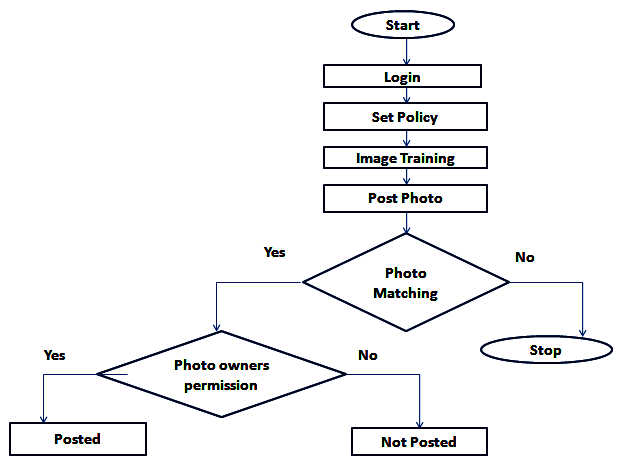
\includegraphics[scale=1]{flowgraph.png}
 % \caption[Proposed System Flow Graph]{Proposed system flow graph}
 % \label{pf}
%\end{figure}
%%%%%%%%%%%%%%%%%%%%%%%555
\vspace{2cm}
\begin{figure}[H]
\begin{minipage}[c]{1\linewidth}
\begin{center}
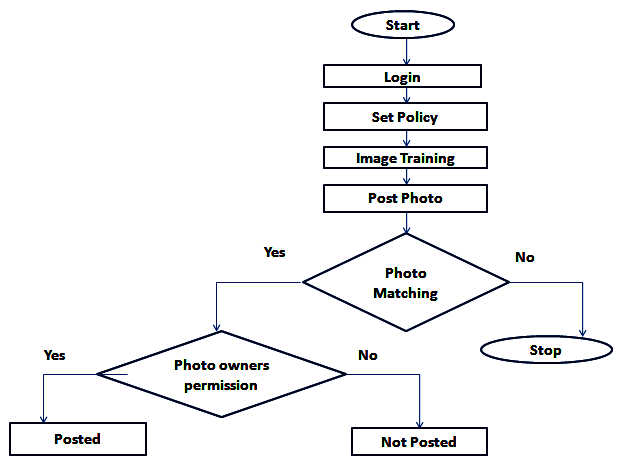
\includegraphics[width=\textwidth]{flowgraph.png}
           % \text{\scriptsize(ISO 9001:2008 Certified)}
           \caption[Proposed System Flow Graph]{ Proposed system flow graph}
             \label{Posted }
\end{center}
  \end{minipage}            
\end{figure}
%%%%%%%%%%%%%%%%%%%%%%%%%%%%%%%%%%
The flow graph shown in figure 4.2 shows  the entire flow of proposed system clearly.Start with user login,Image training, policy setting,photo uploadind, notification sending and Finally collect the decision from each co-photo owners, if all are agreed to upload the  image,then  photo posting is granted else not granted.
\clearpage
\section[Proposed Algorithm]{\fontsize{14}{12}\selectfont PROPOSED ALGORITHM}
\subsection[CBIR Algorithm:]{CBIR Algorithm:}
\begin{algorithm}

\caption{CBIR Algorithm to  retrieve most similar image for query image}
   Input: Query image\\
   Output:Most similar image to  the input image\\
\begin{algorithmic}[1]
\State Give input image which contain one or more faces
\State Detecting all faces in the image.
\State Extract the feature vector for the input image 
\State Calculate the weighted features vectors for the input image
\State Calculate the distance between the input image and the centroid            of each K-mean  cluster  and find  the smallest distance

\State Calculate the distance between the input image and the images
            in the cluster that has the smallest distance with
             the    input image

\State Retrieve   most similar image to the input image  and Send acceptance 
            notification to co -photo owners within the close circle.


\end{algorithmic}
\end{algorithm}

% % \nointent
  \vspace*{1pc}
CBIR algorithm is used for face recognition in the proposed system.CBIR algorithm is one of the most popular algorithm used for image retrieval.The proposed system  using Haar cascade classifier for face detection,it crops all the face regions from the images ,so need not find the similarity based on global feature.in the proposed algorithm we are  giving face images  which is croped using  Haar cascade classifier to the CBIR system , then find  the feature vector for each and calculate  Euclidean distance to get most matching image ,the image which is already trained and saved in cluster files.Our proposed scheme be  very useful in protecting users’ privacy in photo/image sharing over OSNs.
\clearpage

\section[System Designs]{\fontsize{14}{12}\selectfont SYSTEM DESIGNS}
%4.2 SYSTEM DESIGNS	
This section explains various designs used for the project,they are use case diagrams of admin and user, admin's and user's data flow diagrams.These diagrams help to understand the entire operations of the system.This section also explains various tables used for the project.The relational database management system MySql server is used for this purpose.

\subsection[Use Case Diagrams]{Use Case Diagrams}
In this Project there are mainly two parts user and admin. Use case diagram  of admin shown in figure 4.3.Admin can login with a valid password, once login admin can view the user detals like username, profile picture, email id, mobile phone number, moreover admin can do the performance analysis. Performance analysis is done based on time taken (mille seconds)to train an  image, face detection and face recognition. It can be  displayed using a bar chart.  main function of admin is to train the user image and saving values corresponding to each image in a cluster file for later search process
\begin{figure}[H]
 \centering
  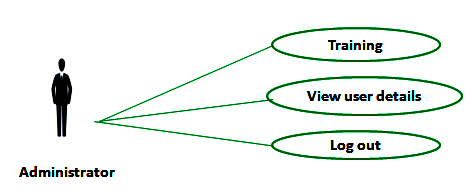
\includegraphics[scale=0.8]{au.png}
  \caption[Admin:Use Case Diagram]{Admin:Use case diagram}
  \label{pf}
\end{figure}
%%%%%%%%%%%%%%%5
This project is based on social networking platform, so most of the operations are done by user. Use case diagram  of user is  shown in figure 4.4.In this system an  individual can create an account using “new registration option”, then user can login with a valid username and password, user can select his/ her image for taining purpose, once image selected admin will do the training process. User can choose friends by using invite friend option. Policy setting is an important part in this project, if user is selecting the notification checkbox then only he/she will get the notification whenever somebody is trying to upload his / her photo. Photo uploading is the main part done by user, here face detection and recognition is take part.
\begin{figure}[H]
 \centering
  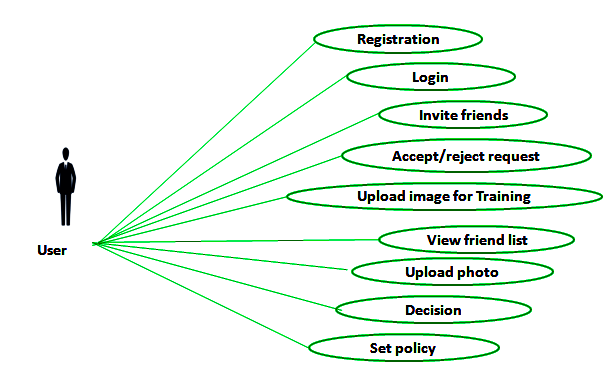
\includegraphics[scale=0.8]{uu.png}
  \caption[User:Use Case Diagram]{User:Use case diagram}
  \label{pf}
\end{figure}
\subsection[Data Flow Diagrams]{Data flow diagrams}
\noindent
\justifying
This section discuss the design of the proposed system.Figure 4.5 gives the descriptions of the notations used in the flow diagram.Rectangle represents an entity, a source of data or destination for data.Processes are the tasks that are performed by the system.Label the arrows with the name of the data that moves through it.Data stores are repositories of data in the system.
%%%%%%%%%%%%%%%%%%%%%%%%%%%%%%%
 \begin{figure}[H]
 \centering
  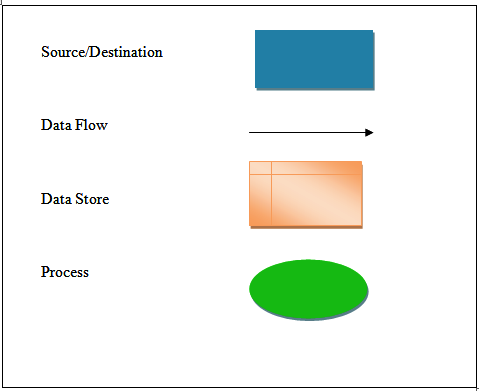
\includegraphics[scale=1]{ndfd0.png}
  \caption[Data Flow Diagram Notations]{Data flow diagram notations}
  \label{pf}
\end{figure}
%%%%%%%%%%%%%%%%%%%%%%%%55

\begin{figure}[H]
\begin{minipage}[c]{1\linewidth}
\begin{center}
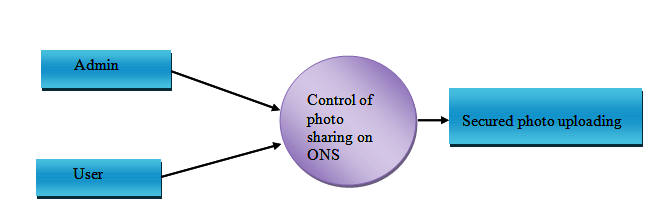
\includegraphics[width=\textwidth]{ndfd1.png}
           % \text{\scriptsize(ISO 9001:2008 Certified)}
         \caption[Context Level DFD]{ Context level DFD}
             \label{Posted photo on time line of Social Networking site}
\end{center}
  \end{minipage}            
\end{figure}
%%%%%%%%%%%%%%%%%%%
\begin{figure}[H]
\begin{minipage}[c]{1\linewidth}
\begin{center}
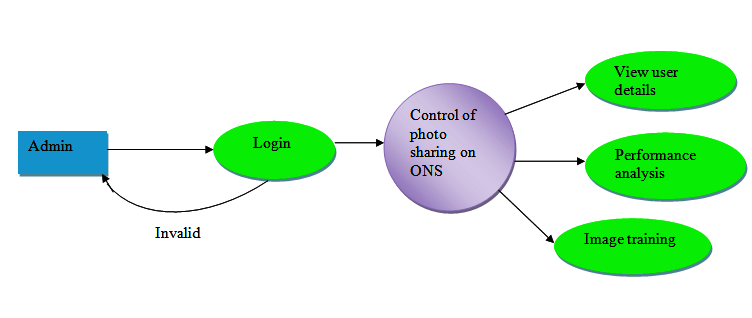
\includegraphics[width=\textwidth]{ndfd2.png}
           % \text{\scriptsize(ISO 9001:2008 Certified)}
        \caption[Admin: level 0 DFD]{ Admin: Level 0 DFD}
             \label{Posted photo on time line of Social Networking site}
\end{center}
  \end{minipage}            
\end{figure}
%%%%%%%%%%%%%%%%%%%%%%%%%%%
\begin{figure}[H]
\begin{minipage}[c]{1\linewidth}
\begin{center}
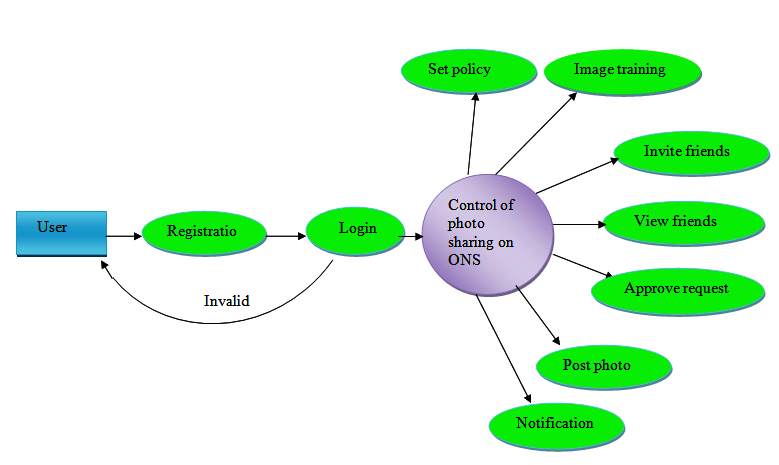
\includegraphics[width=\textwidth]{nndfd2.png}
           % \text{\scriptsize(ISO 9001:2008 Certified)}
           \caption[User: level 0 DFD]{ User: Level 0 DFD}
             \label{Posted photo on time line of Social Networking site}
\end{center}
  \end{minipage}            
\end{figure}
%%%%%%%%%%%%%%%%%%%%%%
\begin{figure}[H]
\begin{minipage}[c]{1\linewidth}
\begin{center}
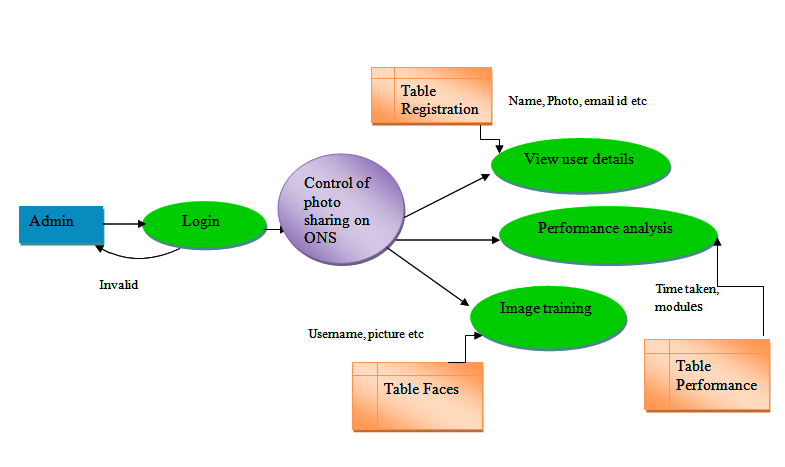
\includegraphics[width=\textwidth]{ndfd4.png}
           % \text{\scriptsize(ISO 9001:2008 Certified)}
           \caption[Admin: Level 1 DFD]{ Admin: Level 1 DFD}
             \label{Posted photo on time line of Social Networking site}
\end{center}
  \end{minipage}            
\end{figure}
%%%%%%%%%%%%%%%
\begin{figure}[H]
\begin{minipage}[c]{1\linewidth}
\begin{center}
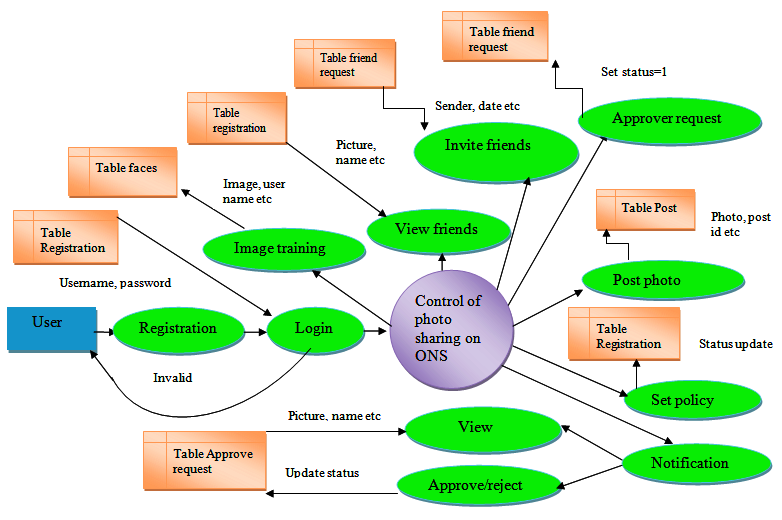
\includegraphics[width=\textwidth]{nndfd5.png}
           % \text{\scriptsize(ISO 9001:2008 Certified)}
            \caption[User: Level 1 DFD]{ User: Level 1 DFD}
             \label{Posted photo on time line of Social Networking site}
\end{center}
  \end{minipage}            
\end{figure}
\clearpage
%%%%%%%%%%%%%%%%

%%%%%%%%%%%%%%%%%%%%%%%%%%
%\subsection[TB]{Table designs}
\subsection{Table design}
The project require a database for storing details of admin and users  and their operations.This section also explains various tables used for the project.The relational database management system MySql server is used for this purpose.The databse is constantly updated and maintained.

% % \nointent
  \vspace*{1pc}
The database table "approve request" shown in figure 4.11 is used  when a user is uploading a photo using post photo option a post id will be generated , photo uploader name will be added to  the column” From user “ and all the recognized persons who need to get the notifications will be added to the column “ To user”.Initially status will be zero ,any one is accepting the notification then  corresponding status value will be changed to one and any one is  rejecting the notification  then corresponding status will be changed to two.
\begin{figure}[H]
\begin{minipage}{1\linewidth}
\centering
%\begin{center}
 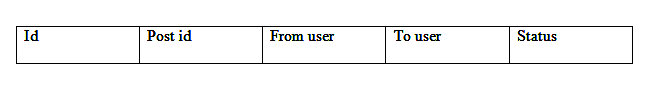
\includegraphics[width=\textwidth]{tb1.png}
           % \text{\scriptsize(ISO 9001:2008 Certified)}
            \caption[Approve Request Table]{Approve request table}
             \label{art}
%\end{center}
\end{minipage}
\end{figure}
% \nointent
\justifying
The database table image training shown in figure 4.12 is used to add details while a user upload his/her photos for training purpose. Initially   values in status column are  zero for all registered users ,once training   is done successfully selected photo for training will be added to the table and status will be updated to the value one.
\begin{figure}[H]   
\begin{minipage}{1\linewidth}
\centering
%\begin{center}
 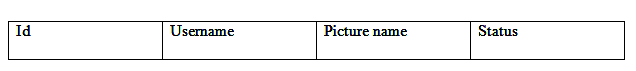
\includegraphics[width=\textwidth]{tb2.png}
           % \text{\scrize(ISO 9001:2008 Certified)}
            \caption[Image Training Table]{Image training table}
             \label{itt}
%\end{center}
\end{minipage}
\end{figure}
% \nointent
\justifying
The database table" friend request" is shown in figure 4.13 is used when a user is sending a friend request to anyone in this project, then the sender’s and receiver’s name will be added to the friend request table .  Initially  values in the status column will be zero and if the receiver is accepting the friend request, status will be changed to the value one.
\begin{figure}[H]
\begin{minipage}{1\linewidth}
\centering
%\begin{center}
 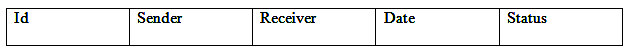
\includegraphics[width=\textwidth]{tb3.png}
           % \text{\scriptsize(ISO 9001:2008 Certified)}
            \caption[Friend Request Table]{Friend request table}
             \label{frt}
%\end{center}
\end{minipage}
\end{figure}
% \nointent
\justifying
The data base table "post" shown in figure 4.14 is used when an user  is posting  a photo, then username , photo used to upload and date of attempt will be added to the table .Initially status will be zero and once the photo is posted, then status will be changed to one.
\begin{figure}[H]
\begin{minipage}{1\linewidth}
\centering
%\begin{center}
 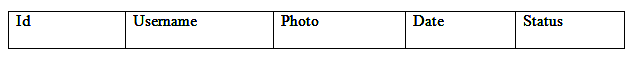
\includegraphics[width=\textwidth]{tbl5.png}
           % \text{\scriptsize(ISO 9001:2008 Certified)}
            \caption[Table Photo Post]{ Table photo post}
             \label{pt}
%\end{center}
\end{minipage}
\end{figure}
% \nointent
\justifying
The data base table "registration" shown in figure 4.15 is used when a person is registering with social networking system,  All user details will be added to this registration table. Here” username” set as primary key. In this table 4.5 privacy policy indicates set of users  who can access the photo , value will be zero if the user selecting” public view” option and the value  will be one if user selecting  “view to my friends” option, if notification policy is selected by user then the corresponding value in the database table will be one otherwise zero.
\begin{figure}[H]
\begin{minipage}{1\linewidth}
\centering
%\begin{center}
 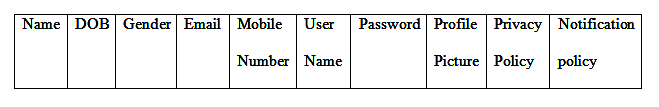
\includegraphics[width=\textwidth]{tbl7.png}
           % \text{\scriptsize(ISO 9001:2008 Certified)}
            \caption[Registration Table]{Registration table}
             \label{rt}
%\end{center}
\end{minipage}
\end{figure}
%%%%%%%%%
% \nointent
\justifying
The data base table "face cutter" shown in figure 4.16 is used when the user is uploading a photo, image will be added to the table ,and no of detected faces in the   photo is added to the” count”  field.
\begin{figure}[H]
\begin{minipage}{1\linewidth}
\centering
%\begin{center}
 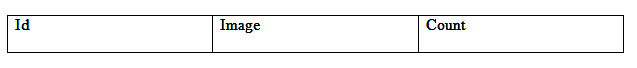
\includegraphics[width=\textwidth]{tbl8.png}
           % \text{\scriptsize(ISO 9001:2008 Certified)}
            \caption[Face Cutter Table]{Face cutter table}
             \label{ft}
%\end{center}
\end{minipage}
\end{figure}

\clearpage
%%%%%%%%%%%%%%%%%%%%%%%[ MODIFICATION ]%%%%%%%%%%%%%%%%%%%%%%%%%%%%%%
%%%%%%%%%%%%%%%%%%%%%%%[ task setup ]%%%%%%%%%%%%%%%%%%%%%%%%%%%%%%
%\addtocontents{toc}{\cftpagenumberson{chapter}}
\chapter[TASK SETUP AND IMPLEMENTATION]{\fontsize{16}{12}\selectfont RESULT AND DISCUSSION}
\section[Modules]{\fontsize{14}{12}\selectfont MODULES}
\subsection[Admin Module]{Admin module}
%\begin{description}
  \begin{description}
\item [(i)]Image training.
%\end{description}
\begin{enumerate}
  \item Face detection.
   \item Image decomposition.
   \item Feature extraction.
   \item Clustering.
\end{enumerate}
\end{description}
\subsection[User Module]{User module}
\begin{description}
\item [(ii)]Photo uploading
\begin{enumerate}
  \item Face Detection.
   \item Face recognition and send notification. 
  \end{enumerate}
\end{description}
\clearpage
\section[System Requirements]{\fontsize{14}{12}\selectfont SYSTEM REQUIREMENTS}
%%%%%%%%%%%%%%%%%%%%%%%%
\begin{table}[H]
\centering
\caption{Software requirement }
\vspace*{.5cm}
\label{routing}
\begin{tabular}{|c|c|}
\hline
\textbf{Parameter} &\textbf{Used for project}        \\
\hline
Operating System  &Windows 8          \\
      
\hline
IDE &NetBeans 7.4            \\
 \hline
Front End &Java7.0 and JSP 2.4          \\
\hline
Back End &MySQL5.0           \\
 \hline
Application Server &Apache Tomcat7.0.41            \\

\hline
\end{tabular}
\end{table}
%%%%%%%%%%%%%%%%%%%%%%%%%%
%%%%%%%%%%%%%%%%%%%%%%%%
\vspace*{1cm}
\vspace*{1cm}
\begin{table}[H]
\centering
\caption{Hardware requirement }
\vspace*{.5cm}
\label{routing}
\begin{tabular}{|c|c|}
\hline
\textbf{Parameter} &\textbf{Used for project}        \\
\hline
Processor &Intel(R)Celeron(r)CPU N2830          \\
      
\hline
Speed&2.16GHz           \\
 \hline
RAM &4GB         \\
Hard Disk &360GB           \\

\hline
\end{tabular}
\end{table}
%%%%%%%%%%%%%%%%%%%%%%%%%%%%%%%



%%%%%%%%%%%%%%%%%%%%%%%[ task setup ]%%%%%%%%%%%%%%%%%%%%%%%%%%%%%%
%\addtocontents{toc}{\cftpagenumberson{chapter}}
\chapter[RESULT AND DISCUSSION]{\fontsize{16}{12}\selectfont RESULT AND DISCUSSION}
\section[Result]{\fontsize{14}{12}\selectfont RESULT}
\noindent
Careless photo posting may reveal privacy of individual in a posted photo. This result enables individuals potentially in a photo to give the permissions before posting a co-photo. I successfully  designed   and tested a privacy-preserving FR system to identify individuals in a co-photo. The proposed system is featured with low computation cost and confidentiality of the training set. Theoretical analysis and experiments were conducted to show effectiveness and efficiency of the work.

% % \nointent
  \vspace*{1pc}
To achive this goal i used CBIR algorithm with K- Mean clustering. The main target of CBIR is to get accurate results with lower computational time.I hope i have done the project with accurate result and lower computational cost.Careless photo posting may reveal privacy of individual in a posted photo. This project result enables individuals potentially in a photo to give the permissions before posting a co-photo.Various web pages of this project is given here.
\clearpage
\subsection[User Registration Page]{User registration page}
To exploit the features of this Online Social Networks every users  need to create an account. User can create a user name and password  User registration page is shown in the figure 6.1.
\vspace{1cm} 
\vspace{1cm}
\vspace{1cm}

 \begin{figure}[H]
\begin{minipage}[c]{1\linewidth}
\begin{center}
 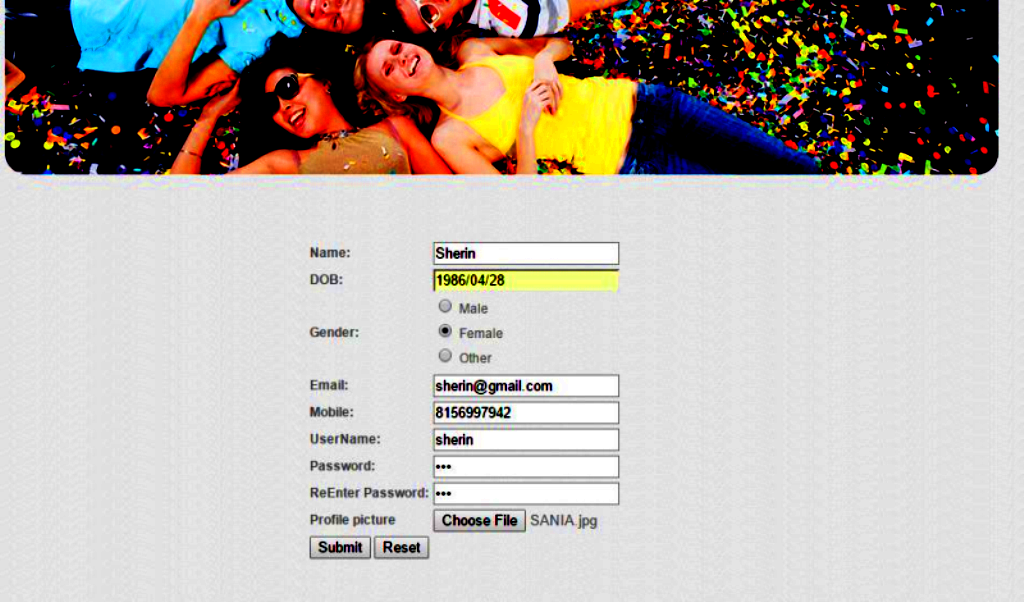
\includegraphics[width=\textwidth]{rej.png}
           % \text{\scriptsize(ISO 9001:2008 Certified)}
        \caption[User Registration Page]{User registration page}
        \label{Login page}
\end{center}
\end{minipage}  
      \end{figure} 
% \clearpage
 \noindent
 \clearpage
 \subsection[Login Page]{Login page}
If registration done successfully user can login to his/her account to explore the features of online social networking.User can login with a valid user name and password.Registration user should enter email id,mobile,number, user name, password etc.Once user login through the page shown in the figure 6.2, then user can use edit profile to edit all the details entered during the  registration time.Administrator can also use the same login page with a valid user name and password.
\vspace{1cm} 
\vspace{1cm}
\vspace{1cm}
\begin{figure}[H]
\begin{minipage}[c]{1\linewidth}
\begin{center}
 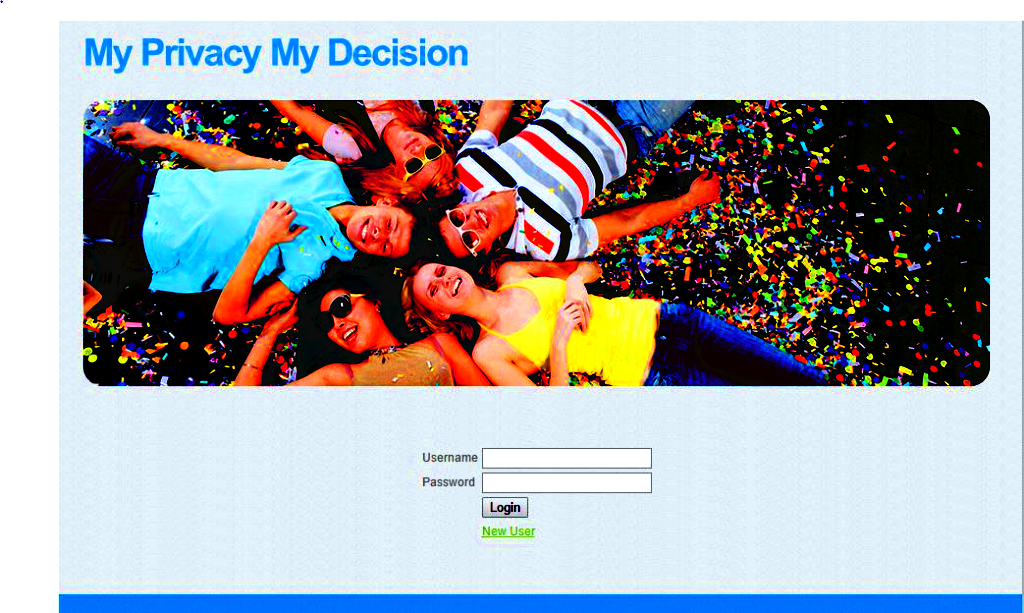
\includegraphics[width=\textwidth]{1.png}
           % \text{\scriptsize(ISO 9001:2008 Certified)}
        \caption[Login Page]{Login page}
        \label{Login page}
\end{center}
\end{minipage}  
      \end{figure} 
% \clearpage
 \noindent
 \clearpage 
 \subsection[Upload Image for Training]{Upload image for training}
Once user login to his /her account then  he/she  can  select an image for training purpose. User should select their own image for training,then only it is possible to get notification while some one else is trying  to upload a photo of them. For better performance user can train the system with more than one images, even using childhood images.User image uploading for training  page is shown in  the figure 6.3.
\vspace{1cm} 
\vspace{1cm}
\vspace{1cm}
\begin{figure}[H]
\begin{minipage}[c]{1\linewidth}
\begin{center}
 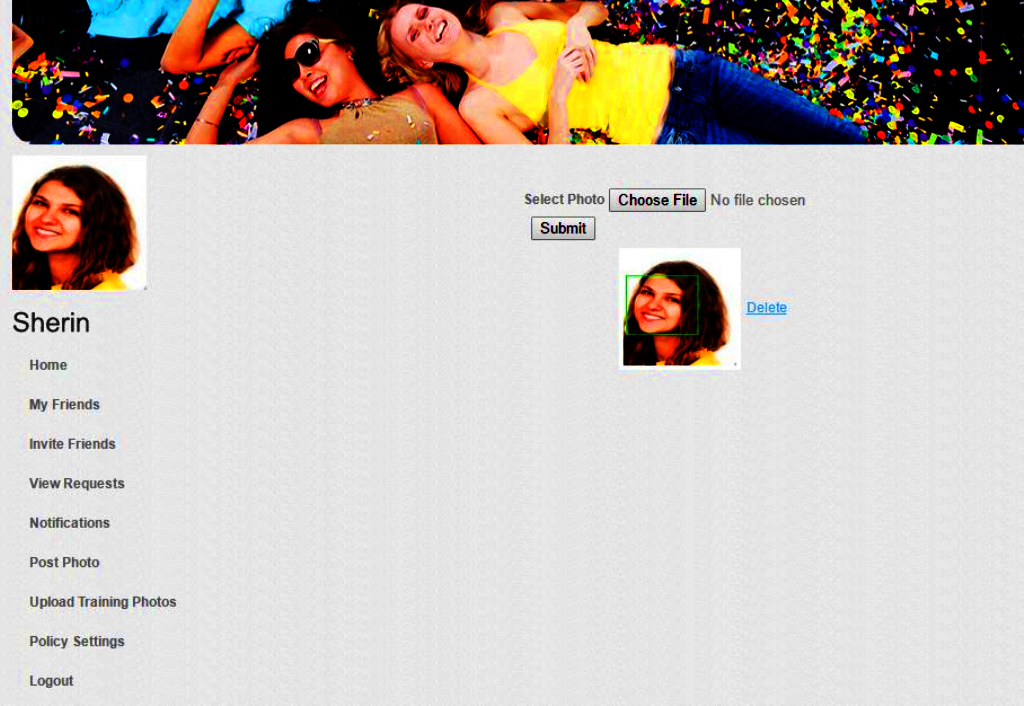
\includegraphics[width=\textwidth]{training2.png}
           % \text{\scriptsize(ISO 9001:2008 Certified)}
      \caption[Upload Image for Training Page]{Upload image for training}
        \label{Upload image for training}
\end{center}

  \end{minipage}  
   
      \end{figure}
      
\clearpage
 \subsection[Image Training Page]{Image training page}
\noindent
Once user select an image and upload it for training, then the notification is going to administrator. Administrator can now train the image.Normally admin is taking six to seven seconds for the training processes.Admin image training  page is shown in the figure 6.4.
\vspace{1cm} 
\vspace{1cm}
\vspace{1cm}
\begin{figure}[H]
\begin{minipage}[c]{1\linewidth}
\begin{center}
 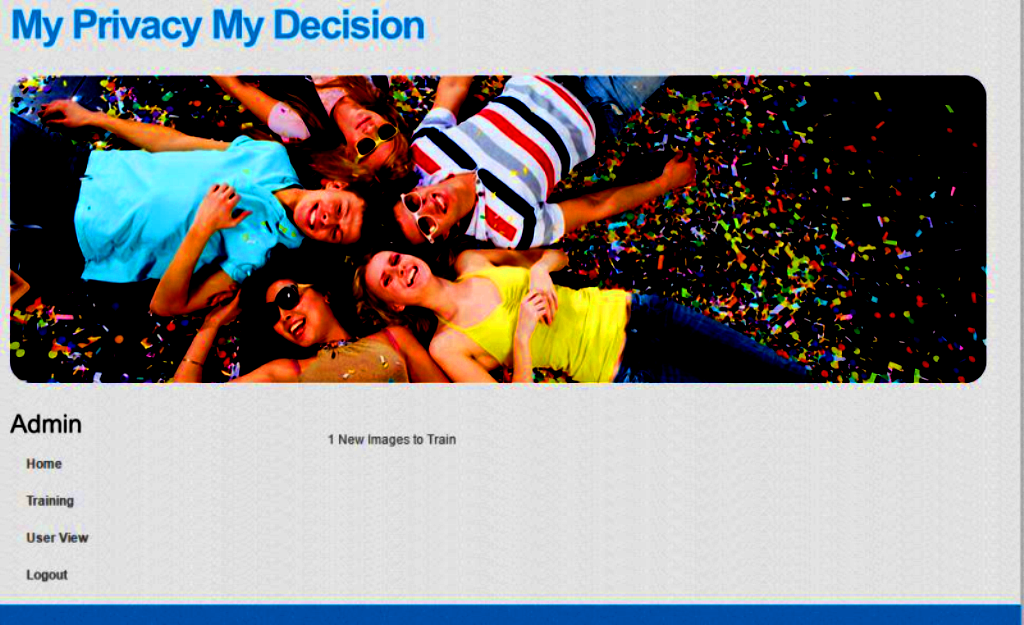
\includegraphics[width=\textwidth]{admintrain.png}
           % \text{\scriptsize(ISO 9001:2008 Certified)}
            \caption[Image Training Page]{Image training page}
             \label{Image training page}
\end{center}
\end{minipage}	
\end{figure}

\clearpage
 \subsection[Invite Friends Page]{Invite friends page}
\noindent
 Once ueser is login with an valid user name and password ,user is able to send a friend request and accept friend request.
To send a friend request user can use invite friend option in the given system, then the name and profile picture with an invite friend option will be displayed and now logged user can invite any one.Invite friends  page is shown in the figure 6.5.
\vspace{1cm} 
\vspace{1cm}
\vspace{1cm}
 
 \begin{figure}[H]
\begin{minipage}[c]{1\linewidth}
\begin{center}
 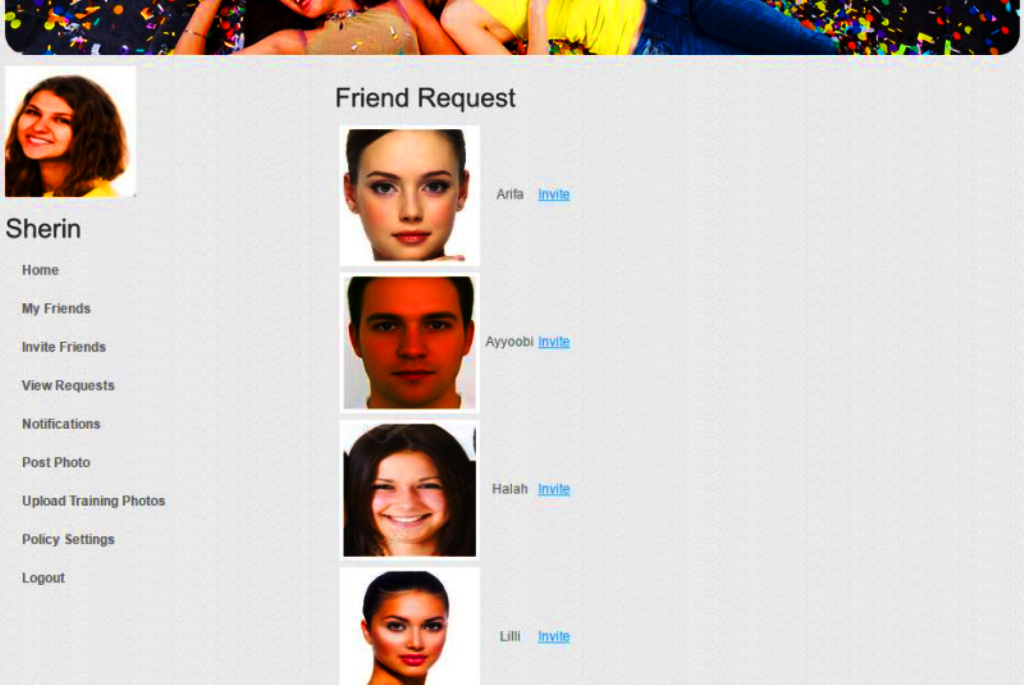
\includegraphics[width=\textwidth]{sherininvitefriends.png}
           % \text{\scriptsize(ISO 9001:2008 Certified)}
            \caption[Invite Friends Page]{Invite friends page.}
             \label{Invite friends}
\end{center}
\end{minipage}
\end{figure}
\clearpage
 \subsection[View Friend Request Page]{View friend request page}
\noindent
 Once user is login with an valid user name and password ,user is able to send a friend request and accept friend request.Logged user can view all  the friend request received by using the option view friend request in this system and user can accept or reject fried request.View friend request page is shown in the figure 6.6.
\vspace{1cm} 
\vspace{1cm}
\vspace{1cm}
 
\begin{figure}[H]
\begin{minipage}[c]{1\linewidth}
\begin{center}
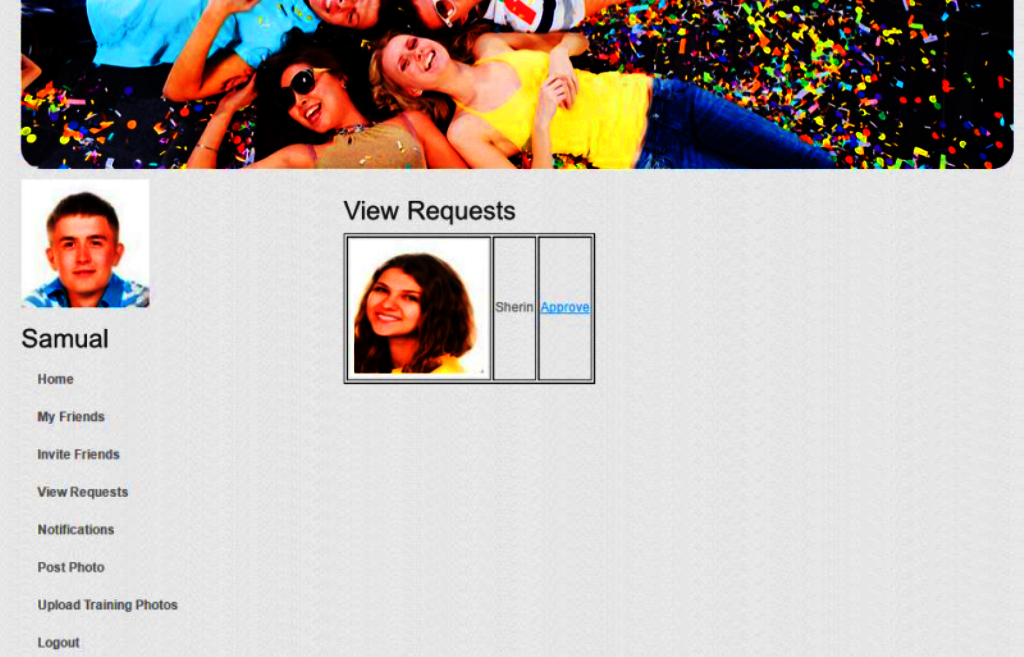
\includegraphics[width=\textwidth]{pendingrequest.png}
           % \text{\scriptsize(ISO 9001:2008 Certified)}
            \caption[View Friend Request Page]{View friend request page}
             \label{View friend request}
\end{center}
\end{minipage}
            
\end{figure}

\clearpage
 \subsection[View Friend List Page]{View friend list page}
 \noindent
 Once user is login with an valid user name and password,user is able to view his/her friend list using the option view friend list in this system.View friend list page is shown in the figure 6.7. 
 \vspace{1cm} 
\vspace{1cm}
\vspace{1cm} 
 
\begin{figure}[H]
\begin{minipage}[c]{1\linewidth}
\begin{center}
 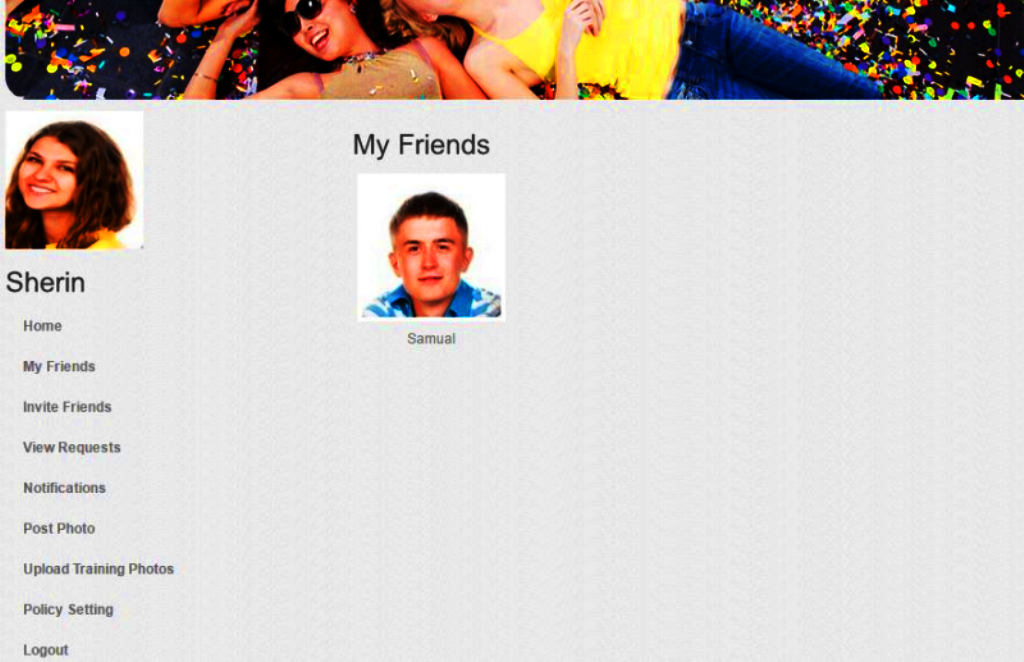
\includegraphics[width=\textwidth]{sherinsfriend.png}
           % \text{\scriptsize(ISO 9001:2008 Certified)}
            \caption[View Friend List Page]{View friend list page}
             \label{Friend list}
\end{center}
 \end{minipage}          
\end{figure}
\clearpage
 \subsection[Post Photo Page]{Post photo page}
\noindent
User can use post photo option in this system to upload any image,to do this user can  browse a   photo from gallery and   upload it by using post photo option.If the image contains human face or faces then Haar cascade  classifier based Face detection  will be activated and cropping all the individual faces from the photo which is being uploading.Post photo page is shown in the figure 6.8. 
 \vspace{1cm} 
\vspace{1cm}
\vspace{1cm}
\begin{figure}[H]
\begin{minipage}[c]{1\linewidth}
\begin{center}
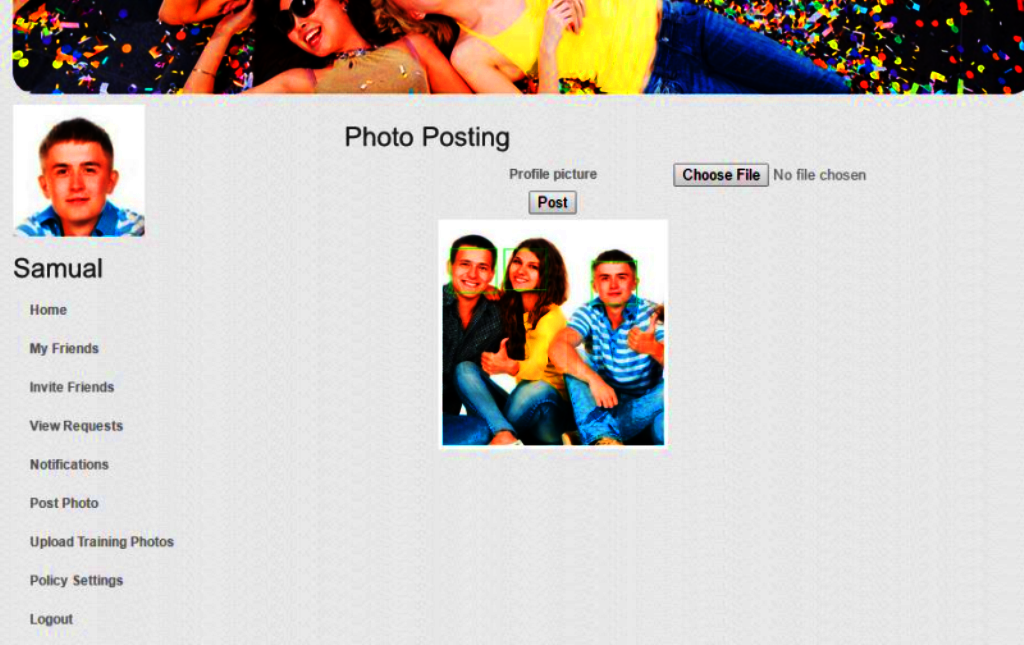
\includegraphics[width=\textwidth]{post.png}
           % \text{\scriptsize(ISO 9001:2008 Certified)}
            \caption[Post Photo Page]{Post photo page}
             \label{Face Detection}
\end{center}
 \end{minipage}           
\end{figure}
\clearpage
 \subsection[Notification Page]{Notification page}
\noindent
When a user try to upload a group photo , all  individual faces will be detected and FR system  cans recognize everyone in the photo. We are using Open CV Haar cascade classifier  for face detection and CBIR algorithm to train individual images and for face recognition. FR system will identify each individual by comparing their face with  trained set of  images,if a match is found,  sending a notification to co photo-owners within close friend circle  informing their presence.Notification page is shown in the figure 6.9. 
 \vspace{1cm} 
\vspace{1cm}
\vspace{1cm}
\begin{figure}[H]
\begin{minipage}[c]{1\linewidth}
\begin{center}
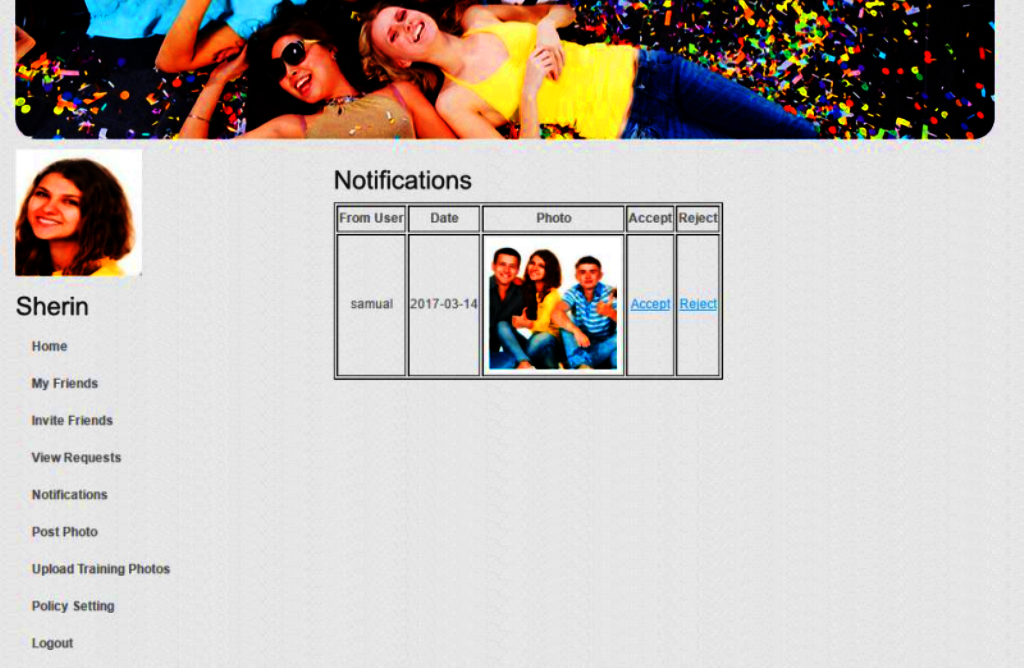
\includegraphics[width=\textwidth]{sherinnew.png}
           % \text{\scriptsize(ISO 9001:2008 Certified)}
            \caption[ Notification Page]{Notification page}
             \label{Notification}
\end{center}
 \end{minipage}             
\end{figure}
\clearpage
 \subsection[ User Time Line Page]{User time line page}
\noindent
If all the notification are accepted by co-photo owners then the  photo will be uploaded  and displayed on the time line page  of  this social networking site.User time line page is shown in the figure 6.10.
\vspace{1cm} 
\vspace{1cm}
\vspace{1cm}
\begin{figure}[H]
\begin{minipage}[c]{1\linewidth}
\begin{center}
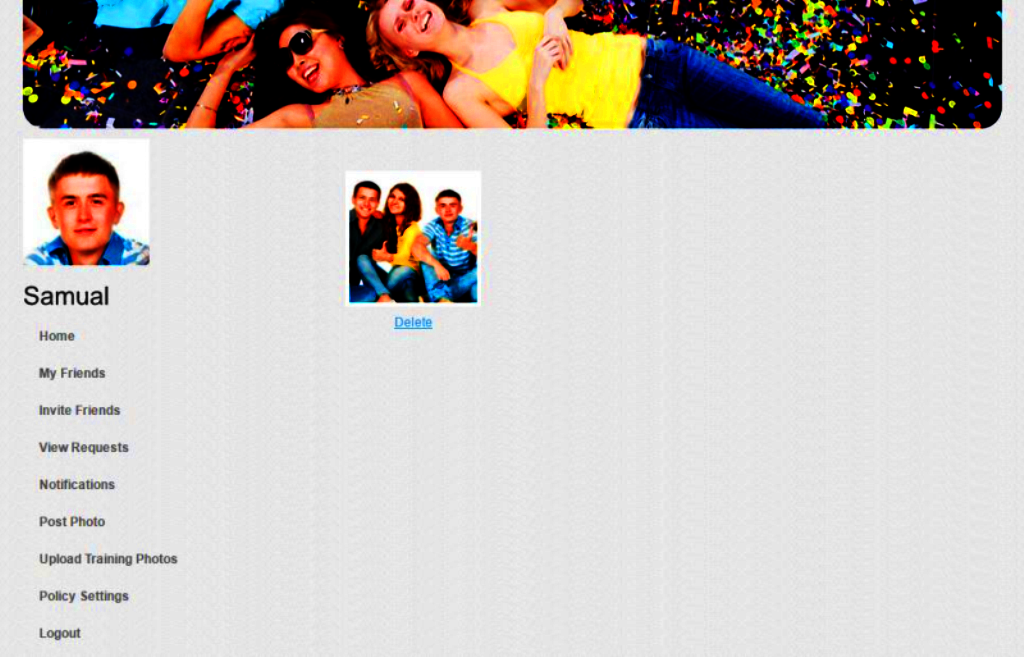
\includegraphics[width=\textwidth]{photoposted.png}
           % \text{\scriptsize(ISO 9001:2008 Certified)}
            \caption[Posted Photo on Time Line of Social Networking Site]{Posted photo on time line of social networking site}
             \label{Posted photo on time line of Social Networking site}
\end{center}
  \end{minipage}            
\end{figure}
\clearpage

\section[DISCUSSION]{\fontsize{14}{12}\selectfont DISCUSSION}
% % \nointent
Control of photo sharing on online social network project work has completed successfully. Various test is conducted during the code generation phase itself. All the errors were rectified at the moment of its discovery. Attention is diverted to individual modules, independently to one another to locate errors.  Registration ,login, photo uploading, privacy policy settings, training individuals images, send and accept friend request ,photo detection, face recognition  and notification acceptance modules tested independently ,this has enabled the detection of errors in coding and logic. To test the efficient working  of  face recognition, we train this system by more than one photos with different  expressions and got successful result.To test the human face detection capability of haar cascade classifier, we tested with various face images, non face images and even with animal faces and got successful result. Finally all these modules are integrated in a master page and tested successfully.

% % \nointent
  \vspace*{1pc}
Careless photo posting may reveal privacy of individual in a posted photo. This result enables individuals potentially in a photo to give the permissions before posting a co-photo. We designed a privacy-preserving FR system to identify individuals in a co-photo. The proposed system is featured with low computation cost and confidentiality of the training set. Theoretical analysis and experiments were conducted to show effectiveness and efficiency of the work. I expect that scheme be very useful in protecting users’ privacy in photo/image sharing over online social networks.

\clearpage
 
 
 
\section[PERFORMANCE ANALYSIS]{\fontsize{14}{12}\selectfont PERFORMANCE ANALYSIS}

This section, analyses the overall performance of the proposed system by computing the
performance score for each module in the system. The performance analysis graph is shown in Figure 6.11. The modules used for the performance analysis  are image training, face detection and face recognition.To do performance analysis  starting time and ending time for each modules are calculating, then finding the time difference and storing it in a database table, then plot the performance graph by taking the time from database table. In this graph X-coordinates are various modules used in this system and Y-coordinates are time taken  in seconds used to complete each modules. The observation table of proposed system is  shown in table 6.1.

\begin{figure}[ht]
\begin{minipage}[c]{1\linewidth}

%\end{figure}h]
\begin{center}
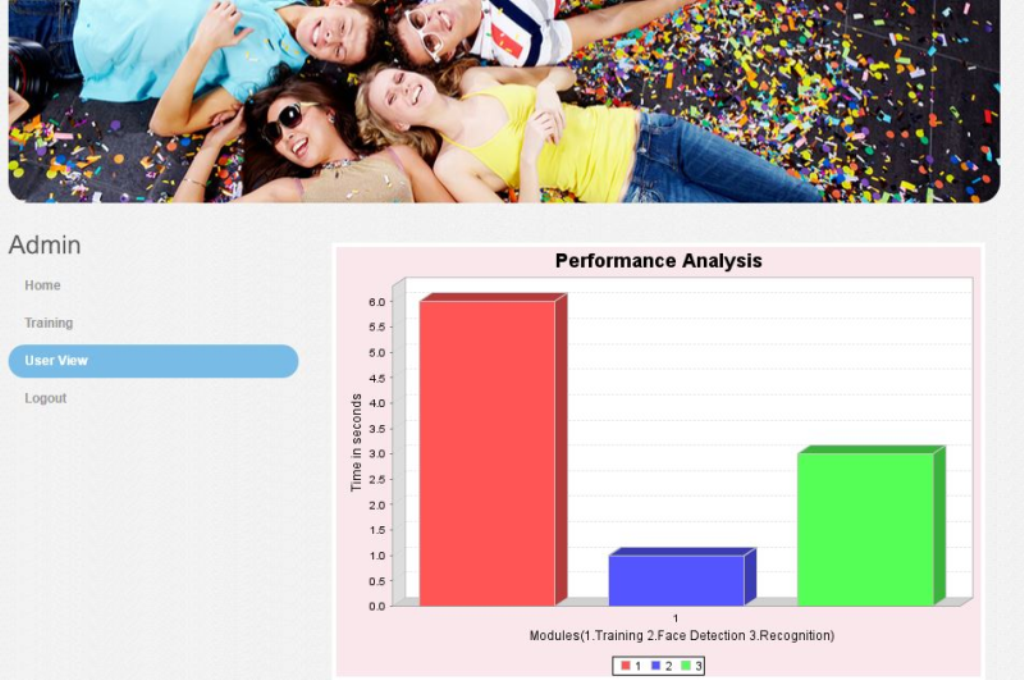
\includegraphics[width=\textwidth]{newperfomance.png}
           % \text{\scriptsize(ISO 9001:2008 Certified)}
            \caption[Performance Analysis Graph]{Performance analysis graph}
             \label{PerformanceAnalysis}
\end{center}
 \end{minipage}          
\end{figure}
\begin{table}[H]
\centering
\caption{Observation table for proposed system}
\label{routing}
\vspace{.5cm}
\begin{tabular}{|c|c|c|}
\hline
\textbf{SNO:} &\textbf{Modules}       &\textbf{Time taken(seconds)}  \\
\hline
1     &Training    &   7      \\
      
\hline
1     &FaceDetection    &   2      \\
      
\hline
4 &Face Recognition&2            \\
\hline
\end{tabular}
\end{table}
\clearpage


\clearpage











%%%%%%%%%%%%%%%%%%%%%%%[ CONCLUSION]%%%%%%%%%%%%%%%%%
%\addtocontents{toc}{\cftpagenumberson{chapter}}

\chapter[CONCLUSION]{\fontsize{16}{12}\selectfont CONCLUSION }

Photo sharing is one of the most popular features in online social networks such as Facebook. Lamentably, imprudent photograph posting may uncover security of people in a posted photograph. To control the security spillage, we proposed to empower people possibly in a photograph to give the consents before posting a co-photograph. We planned a security safeguarding FR framework to recognize people in a co-photograph. The proposed framework is highlighted with low calculation expense and privacy of the preparation set. Hypothetical examination and trials were directed to show adequacy and effectiveness of the proposed plan. We expect that our proposed plan be exceptionally helpful in ensuring clients' protection in photograph/picture sharing over online informal organizations.Our future work could be the way to move the proposed preparing plans to individual mists like Dropbox and/or icloud.Secured video sharing through online social networking will also be our future enhancement. 

 \newpage
 \thispagestyle{empty}
 
%\end{document}
%%%%%%%%%%%%%%%%%%%%%%%%%[ END OF CHAPTERS ]%%%%%%%%%%%%%%%%%%%%%%%%%%%%%%%%%%